\DeclareOption*{\PassOptionsToClass{\CurrentOption}{abntex2}}
\ProcessOptions

\documentclass[
	% -- opções da classe memoir --
	12pt,				% tamanho da fonte
	openright,			% capítulos começam em pág ímpar (insere página vazia caso preciso)\
	oneside,			% para impressão em verso e anverso. Oposto a oneside
	a4paper,			% tamanho do papel. 
	% -- opções da classe abntex2 --
	chapter=TITLE,		% títulos de capítulos convertidos em letras maiúsculas
	%section=TITLE,		% títulos de seções convertidos em letras maiúsculas
	%subsection=TITLE,	% títulos de subseções convertidos em letras maiúsculas
	%subsubsection=TITLE,% títulos de subsubseções convertidos em letras maiúsculas
	% -- opções do pacote babel --
	english,			% idioma adicional para hifenização
	french,				% idioma adicional para hifenização
	spanish,			% idioma adicional para hifenização
	brazil				% o último idioma é o principal do documento
	]{abntex2}

\usepackage{conf-ifsc}	

%---------------------------------------------------------------------%
%---------------------------------------------------------------------%
% Informações de dados para CAPA e FOLHA DE ROSTO
%---------------------------------------------------------------------%
%---------------------------------------------------------------------%

\titulo{Estudo da redução da interferência eletromagnética de um conversor estático do tipo Buck \interleaved}

\autor{Diesson Stefano Allebrandt}

\local{Florianópolis}

\data{2021}

\orientador[Orientador:\\]{Luis Carlos Martinhago Schlichting}

\coorientador[Coorientador:\\]{Joabel Moia}

\tipotrabalho{Monografia (Graduação)}

% O preambulo deve conter o tipo do trabalho, o objetivo, o nome da instituição e a área de concentração 
\preambulo{Trabalho de conclusão de curso submetido ao Instituto Federal de Educação, Ciência e Tecnologia de Santa Catarina como parte dos requisitos para obtenção do título de engenheiro eletrônico}

\textoaprovacao{Este Trabalho foi julgado adequado para obtenção do Título de Engenheiro Eletrônico em março de 2021 e aprovado na sua forma final pela banca examinadora do Curso de Engenharia Eletrônica do instituto Federal de Educação Ciência, e Tecnologia de Santa Catarina.}


%---------------------------------------------------------------------%
% Início do documento
%---------------------------------------------------------------------%

\begin{document}

\selectlanguage{brazil}
\frenchspacing 


% ----------------------------------------------------------
% ELEMENTOS PRÉ-TEXTUAIS
% ----------------------------------------------------------
% \pretextual

\imprimircapa
\imprimirfolhaderosto* %(o * indica que haverá a ficha bibliográfica)

%---------------------------------------------------------------------%
% ATENÇÃO - Pergunte para a Biblioteca do IFSC
% Inserir a ficha bibliografica - 
%
% Para gerar a ficha catalográfica acesse:
% http://ficha.florianopolis.ifsc.edu.br/
% Precisa ser feito pelo navegador Mozilla Firefox
%---------------------------------------------------------------------%

\imprimirficha{pdf/fichacatalografica3.pdf}
\cleardoublepage

%---------------------------------------------------------------------%
% Inserir folha de aprovação
%---------------------------------------------------------------------%

\imprimiraprovacao
\cleardoublepage

%---------------------------------------------------------------------%
% Dedicatória
%---------------------------------------------------------------------%
%\imprimirdedicatoria{Este trabalho é dedicado às crianças adultas que,\\quando pequenas, sonharam em se tornar cientistas.}
% ---

%---------------------------------------------------------------------%
% Agradecimentos
%---------------------------------------------------------------------%
\begin{agradecimentos}
    
    Ao Instituto Federal de Santa Catarina (IFSC), que me proporcionou muitas oportunidades, amizades e crescimento pessoal e profissional. Que através da sua excelente infraestrutura permitiu que esse trabalho fosse possível.
    
    Aos meus familiares e aos muitos amigos que fiz durante a graduação, que me ajudaram e incentivaram durante todo o processo. 
    
    Aos professores, que durante essa jornada me instigaram a sempre buscar por mais e que me proporcionaram trabalhos desafiadores, acreditando no meu potencial. Tais projetos exploraram minhas capacidades e me permitiram expandir limites, o que não seria vivenciado sem a confiança dos docentes.
    
    
    %\marcador{add}{Tanta gente...}
\end{agradecimentos}
% ---

%---------------------------------------------------------------------%
% Epígrafe
%---------------------------------------------------------------------%
\begin{epigrafe}
    \vspace*{\fill}
	\begin{flushright}
		\textit{``Eu não falhei, encontrei 10 mil\\
		soluções que não davam certo.'' \\
		(Thomas A. Edison)}
	\end{flushright}
\end{epigrafe}

%---------------------------------------------------------------------%
% RESUMOS
%---------------------------------------------------------------------%
% resumo em português
\setlength{\absparsep}{18pt} % ajusta o espaçamento dos parágrafos do resumo
\begin{resumo}
    Este trabalho apresenta o estudo de técnicas de compatibilidade eletromagnética para a mitigação do ruído conduzido e irradiado em um conversor estático do tipo Buck \Interleaved. O conversor proposto teve seu projeto iniciado na disciplina de Eletrônica de Potencia e apresenta uma  corrente de saída de \SI{5}{\ampere}, tensão de saída de \SI{5}{\volt} e potência nominal de 25 watts. Neste trabalho, foram realizados os ensaios de emissão conduzida e irradiada do conversor projetado, bem como os ensaios após a aplicação das técnicas propostas, aplicadas de forma isoladas. A fim de ser possível a comparação dos resultados dos ensaios, estabeleceu-se uma padronização dos ensaios, tanto em relação ao posicionamento da placa quanto ao do cabo. Dentre os testes propostos, alguns destacaram-se por apresentar resultados significativos. Uma grande solução apresentada foi a redução da frequência de chaveamento com o uso de um conversor com célula de comutação de três estados. As técnicas testadas de forma isolada não apresentaram melhoras significativas simultaneamente na emissão conduzida e irradiada, porém, ao serem utilizadas de forma combinada, mostraram-se de grande eficácia.
    
    \textbf{Palavras-chave}: Compatibilidade eletromagnética. Eletrônica de potência. Buck \interleaved. Conversor Buck com célula de comutação de três estados.
\end{resumo}

% resumo em inglês
\begin{resumo}[Abstract]
 \begin{otherlanguage*}{english}
    This papper presents the study of electromagnetic compatibility techniques to reduce conducted and irradiated noise in a Buck Interleaved static converter. The proposed converter project had started in the Power Electronics discipline and has an output current of \SI{5}{\ampere}, an output voltage of \SI{5}{\volt} and a 25 watts of nominal power. In this work, the conducted and radiated emission tests of the designed converter were carried out, as well as the tests after the application of the proposed techniques, applied in isolation. In order to be possible to compare the results of the tests, a standardization of the tests was established, related to the position of the board and the cable. Among the proposed tests, some stood out for presenting significant results. A great solution presented was the reduction of the switching frequency with the use of a three-state switching cell converter. The techniques tested in isolation didn't show significant improvements simultaneously in the conducted and irradiated emission, however, when used in combination, they proved to be of great efficiency.

   \vspace{\onelineskip}
 
   \noindent 
   \textbf{Keywords}: Eletromagnetic compatibility. Power eletronics. Buck Interleaved. Three-state switching cell Buck Converter.
 \end{otherlanguage*}
\end{resumo}


%---------------------------------------------------------------------%
% inserir lista de ilustrações
%---------------------------------------------------------------------%
\pdfbookmark[0]{\listfigurename}{lof}
\listoffigures*
\cleardoublepage

%---------------------------------------------------------------------%
% inserir lista de tabelas
%---------------------------------------------------------------------%
%\pdfbookmark[0]{\listtablename}{lot}
%\listoftables*
%\cleardoublepage

%---------------------------------------------------------------------%
% inserir lista de listings
%---------------------------------------------------------------------%
%\pdfbookmark[0]{\lstlistlistingname}{lol}
%\listoflistings
%\cleardoublepage

%---------------------------------------------------------------------%
% inserir lista de abreviaturas e simbolos
%---------------------------------------------------------------------%
%\listofabrev{tex/00-Abreviaturas}
\imprimirlistadeabreviaturas
\imprimirlistadesimbolos
\cleardoublepage

%---------------------------------------------------------------------%
% inserir o sumario
%---------------------------------------------------------------------%
\pdfbookmark[0]{\contentsname}{toc}
\tableofcontents*
\cleardoublepage

% ----------------------------------------------------------
% ELEMENTOS TEXTUAIS
% ----------------------------------------------------------
\textual

% ----------------------------------------------------------
% Inclusão dos capítulos que estão em outros arquivos .tex
% ----------------------------------------------------------

% --- Lista de símbolos ---

\simbolo{\si{\watt}}{watt - Unidade de potência elétrica}
\simbolo{\si{\volt}}{volt - Unidade de potencial elétrico}
\simbolo{\si{\second}}{segundos - Unidade de tempo}
\simbolo{\si{\henry}}{henry - Unidade de indutância}
\simbolo{\si{\ampere}}{ampère - Unidade de corrente elétrica}
\simbolo{\si{\hertz}}{hertz - Unidade de frequência}
\simbolo{\si{\farad}}{farad - Unidade de capacitância}
\simbolo{\si{\ohm}}{ohm - Unidade de resistência elétrica}
\simbolo{\si{\coulomb}}{coulomb - Unidade de carga elétrica}

%%%%%%%%%%%%%%%%%%%%%%%%%%%%%%%%%%%%%%%%%%%%%%%%%%%%%%%%%%%%%%%%%%%
%%%%%%%%%%%%%%%%%%%%%%%%%%%%%%%%%%%%%%%%%%%%%%%%%%%%%%%%%%%%%%%%%%%
\chapter{Introdução}
%%%%%%%%%%%%%%%%%%%%%%%%%%%%%%%%%%%%%%%%%%%%%%%%%%%%%%%%%%%%%%%%%%%
%%%%%%%%%%%%%%%%%%%%%%%%%%%%%%%%%%%%%%%%%%%%%%%%%%%%%%%%%%%%%%%%%%%
    
    Os conversores estáticos são amplamente utilizados em diversas aplicações, como carregadores de bateria de celular, sistema de iluminação, veículos elétricos, sistemas de potência, dentre outros. O uso de conversores estáticos convencionais como \textit{Buck}, \textit{Boost} e \textit{Buck-Boost} apresentam grande usabilidade em muitas aplicações. Porém, para potências mais elevadas, tornam-se menos adequados, uma vez que o aumento da potência nesses conversores acarreta em elementos passivos maiores, sobrecarga nos elementos semicondutores e maior perda de potência, reduzindo sua eficiência \cite{ref:BI_artigo_Falcondes}.
    
    Buscando-se superar essas limitações à medida que a potência desses circuitos aumenta, algumas alternativas são apresentadas, e dentre elas os conversores \interleaved (intercalados). Esses conversores utilizam dois ou mais ramos com elementos ativos em paralelo, para que assim apenas uma fração da corrente total passe por cada semicondutor. Esse processo acaba reduzindo as oscilações e duplicando a frequência de comutação de saída, em um caso com dois ramos paralelos \cite{ref:BI_artigo_Falcondes}.
    
    Por outro lado, devido a natureza dos conversores estáticos ser inerentemente geradora de harmônicos, há uma grande necessidade de estudá-los, uma vez que cada vez mais as aplicações necessitam ser homologadas em normas de \abreviatura&{EMC}{Eletromagnetic Compatibility}{compatibilidade eletromagnética} para que os fabricantes tenham aprovação para a revenda comercial de seus produtos \cite{ref:EMC_artigo_Texas}.
    
    Assim, este trabalho busca verificar o comportamento de um conversor estático \mbox{CC-CC} do tipo Buck \interleaved de dois ramos paralelos do ponto de vista de compatibilidade eletromagnética e aplicar algumas técnicas para a mitigação do ruído presente nesse conversor. Neste trabalho será usada uma norma vigente com a finalidade de facilitar a visualização dos resultados obtidos, porém, não sendo o objetivo deste se adequar a ela.
    
    %%%%%%%%%%%%%%%%%%%%%%%%%%%%%%%%%%%%%%%%%%%%%%%%%%%%%%%%%%%%%%%%%%%
    \section{Justificativa}
    %%%%%%%%%%%%%%%%%%%%%%%%%%%%%%%%%%%%%%%%%%%%%%%%%%%%%%%%%%%%%%%%%%%
        
        % Seria interessante contextualizar algumas aplicações do conversor Buck interleaved, pois qual é a necessidade de se estudar tais técnicas em um conversor que talvez não se use? Teria que ver onde se enquadra as aplicações para tornar atrativo tal estudo
        
        Devido à preocupação dos fabricantes para que seus produtos tenham homologação perante as normas de EMC para obter permissão de comercialização, faz-se importante o estudo de conversores estáticos do ponto de vista de compatibilidade eletromagnética.
        
        Segundo \citeonline{ref:BI_phd_Peraca}, no que diz respeito a conversores estáticos, dentre as estratégias utilizadas em conversores que operam com elevadas correntes, tem-se a técnica do interleaving. Assim, torna-se importante o estudo de EMC de tal conversor, realizando uma análise do ruído conduzido e irradiado gerado por tal estrutura, bem como uma análise de possíveis técnicas para a mitigação desse ruído.
        Sendo esse conhecimento de grande valia, tanto para o meio acadêmico quanto para a indústria.
        
    %%%%%%%%%%%%%%%%%%%%%%%%%%%%%%%%%%%%%%%%%%%%%%%%%%%%%%%%%%%%%%%%%%%
    \section{Descrição do problema}
    %%%%%%%%%%%%%%%%%%%%%%%%%%%%%%%%%%%%%%%%%%%%%%%%%%%%%%%%%%%%%%%%%%%
        
        O conversor Buck \interleaved, por se tratar de um conversor estático de potência, produz harmônicos, principalmente devido a comutações dos semicondutores. Em geral, esses harmônicos se propagam por diferentes meios, tanto por uma conexão elétrica quanto pelo ar, podendo provocar o mal funcionamento em outros equipamentos e a si próprio. Para se evitar a geração e propagação de harmônicos, faz-se importante a aplicação de técnicas ou conjuntos de técnicas de mitigação da interferência eletromagnética.
        
        % O conversor Buck \interleaved, por se tratar de um conversor estático de potência, apresenta ruídos, principalmente devido a comutações dos semicondutores. Em geral, esse ruído se propaga por diferentes meios, tanto por uma conexão elétrica quanto pelo ar, podendo provocar interferência eletromagnética em outros equipamentos e a si próprio. 
        
        %\marcador{alterar}{Assim, o uso de técnicas como a remoção dos dissipadores do circuito, alteração dos tempos de subida no chaveamento dos transistores, uso de um ferrite \textit{bead} e reposicionamento dos elementos magnéticos (indutores) são muitas vezes utilizadas para a redução da interferência eletromagnética em conversores estáticos, por confinar o ruído dentro do conversor chaveado e/ou do componente gerador.}
        
        Dessa forma, a questão-problema que orienta este Trabalho de Conclusão de Curso é: Quais técnicas podem ser aplicadas e qual a eficácia dessas técnicas para a redução da interferência eletromagnética em um conversor estático do tipo Buck \interleaved?
        
    
    %%%%%%%%%%%%%%%%%%%%%%%%%%%%%%%%%%%%%%%%%%%%%%%%%%%%%%%%%%%%%%%%%%%
    \section{Objetivo geral}
    %%%%%%%%%%%%%%%%%%%%%%%%%%%%%%%%%%%%%%%%%%%%%%%%%%%%%%%%%%%%%%%%%%%
    
        Analisar quais técnicas podem ser aplicadas e qual a eficácia dessas técnicas para a redução de interferência eletromagnética em um conversor estático do tipo Buck \interleaved.
    
        %Analisar se o conversor estático do tipo Buck \interleaved pode ser utilizado com técnicas de \marcador*{alterar}{redução da interferência eletromagnética.}{melhorar o objetivo}
        % o uso de técnicas de redução de ruído \marcador*{alterar}{conduzido e irradiado}{EMI} em um conversor estático do tipo Buck \interleaved.
    
    %%%%%%%%%%%%%%%%%%%%%%%%%%%%%%%%%%%%%%%%%%%%%%%%%%%%%%%%%%%%%%%%%%%
    \section{Objetivos específicos}
    %%%%%%%%%%%%%%%%%%%%%%%%%%%%%%%%%%%%%%%%%%%%%%%%%%%%%%%%%%%%%%%%%%%
    
        Com o objetivo geral apresentado, destaca-se os seguintes objetivos específicos: 
    
        \begin{alineas}
            %\item conceituar conversores estáticos;
            
            \item revisar a bibliografia referente a Buck \interleaved, apresentando a forma de funcionamento do circuito, vantagens e desvantagens;
            
            \item conceituar compatibilidade eletromagnética, formas de geração de ruído e técnicas para mitigação;
            
            \item projeto do conversor Buck \interleaved;
            
            %\item análise do circuito e placa de circuito impresso do conversor;
            
            \item análise do ponto de vista de compatibilidade eletromagnética do conversor Buck \interleaved;
            
            \item aplicação de técnicas para mitigação da interferência eletromagnética e análise dos resultados obtidos.
            
        \end{alineas}

%%%%%%%%%%%%%%%%%%%%%%%%%%%%%%%%%%%%%%%%%%%%%%%%%%%%%%%%%%%%%%%%%%%
%%%%%%%%%%%%%%%%%%%%%%%%%%%%%%%%%%%%%%%%%%%%%%%%%%%%%%%%%%%%%%%%%%%
\chapter{Fundamentação Teórica} \label{cap:fund}
%%%%%%%%%%%%%%%%%%%%%%%%%%%%%%%%%%%%%%%%%%%%%%%%%%%%%%%%%%%%%%%%%%%
%%%%%%%%%%%%%%%%%%%%%%%%%%%%%%%%%%%%%%%%%%%%%%%%%%%%%%%%%%%%%%%%%%%
    
    < Texto da Fundamentação Teórica >


\chapter{Metodologia}
    
    Este trabalho busca apresentar e estudar os possíveis problemas de interferência eletromagnética em conversores estáticos e possíveis soluções para a mitigação dos mesmos. Dessa forma, essa pesquisa pode ser classificada como exploratória com abordagem qualitativa. 
    
    Segundo \citeonline[p.~41]{ref:MEP_livro_gil}, uma pesquisa exploratória ``têm como objetivo proporcionar maior familiaridade com o problema, com vistas a torná-lo mais explícito ou a constituir hipóteses''. Já a abordagem qualitativa, para \citeonline[p.~111]{ref:MEP_livro_malhotra}, consiste em uma ``metodologia de pesquisa não estruturada e exploratória baseada em pequenas amostras que proporciona percepções e compreensão do contexto do problema''.
    
    Neste trabalho foi utilizado o \textit{software} KiCad para o projeto do \textit{layout} da placa de circuito impresso, a linguagem de programação Python para o cálculo dos elementos de filtro do conversor e para a geração de todos os gráficos utilizando dados obtidos nos ensaios de EMC e planilhas no \textit{software} SMath para o dimensionamento dos elementos magnéticos.
    
    Desenvolvida a PCB, foram realizados testes elétricos com o objetivo de validar os requisitos de projeto. Nesta etapa, utilizou-se equipamentos de medição como multímetro, osciloscópio, sonda diferencial de alta tensão e sonda de corrente de alta frequência. 
    
    Após validações da parte elétrica do conversor, realizou-se os testes de compatibilidade eletromagnética de emissão conduzida e emissão irradiada. Para as medidas de emissão conduzida, utilizou-se a LISN R\&S ENV216 em conjunto com o analisador de espectro R\&S HMS-X. Nas medida de emissão irradiada, foi utilizado uma câmara GTEM EMCTEST GTEM-750 e o receptor de EMI R\&S ESL3. 
    
    Todas as técnicas de mitigação de EMI testadas foram feitas de forma isolada, para que seja possível analisar o impacto da mesma sem interferência das técnicas anteriormente testadas. Por fim, foi realizado um teste com as técnicas combinadas que obtiveram melhores resultado na redução da EMI. Em todas as medidas utilizou-se como referência a norma CISPR22 classe B com a finalidade de facilitar a visualização dos resultados, porém, não é o objetivo desse trabalho se adequar a ela. 

    
% ----------------------------------------------------------------------- %
% Arquivo: 04-Resultados.tex
% ----------------------------------------------------------------------- %

\chapter{Projeto e resultados}
\label{cap:resultados}

Neste capítulo será abordado o projeto do conversor Buck \interleaved de dois ramos proposto e, em seguida, apresentado medidas da EMI no conversor e possíveis técnicas aplicáveis para a redução da EMI produzida. 
    
    %%%%%%%%%%%%%%%%%%%%%%%%%%%%%%%%%%%%%%%%%%%%%%%%%%%%%%%%%%%%%%%%%%%
    \section{Projeto do conversor Buck \Interleaved de dois ramos} \label{cap:result_proj}
    %%%%%%%%%%%%%%%%%%%%%%%%%%%%%%%%%%%%%%%%%%%%%%%%%%%%%%%%%%%%%%%%%%%
    
    Para o estudo do conversor proposto, sendo iniciado na disciplina de Eletrônica de Potência I, definiu-se algumas especificações de projeto, conforme \autoref{tab:requisitos_buck}.
        
    \begin{table}[htbp]
        \centering
        \caption{Especificações de projeto do conversor Buck \Interleaved de dois ramos}
        \label{tab:requisitos_buck}
        \begin{tabular}{@{}|m{0.50\textwidth}|m{0.15\textwidth}|m{0.10\textwidth}|@{}}
            \hline
             & Valor & Unid. \\
            \hline
            Tensão de entrada               & 24    & \si{\volt}      \\ \hline
            Tensão de saída                 & 5     & \si{\volt}      \\ \hline
            Variação da tensão de saída     & 1     & \si{\percent}    \\ \hline
            Corrente de saída               & 5     & \si{\ampere}     \\ \hline
            Variação da corrente do indutor & 100   & \si{\percent}    \\ \hline
            Frequência de chaveamento       & 50    & \si{\kilo\hertz} \\ \hline
        \end{tabular}
        \indentedfont[0.84\textwidth]{Elaboração própria (2021)}
    \end{table}
    
    Com essas especificações, torna-se possível calcular os componentes de filtro do conversor, utilizando a \autoref{eq:buck_indutor} e a \autoref{eq:cbi_capacitor}. Assim, é obtido o valor de indutância de \SI{31}{\micro\henry} e uma capacitância de \SI{46}{\micro\farad}. A \autoref{fig:esquematico_cbi} apresenta o esquemático desenvolvido no \textit{software} KiCad para a estrutura proposta. Nesse circuito, foi utilizado o \abreviatura.{CI}{circuito integrado} SG3525 para o acionamento dos transistores e adicionados alguns capacitores de filtro de alta frequência (C3, C4, C5 e C7) como boas práticas no desenvolvimento de um \textit{Layout}. Os indutores em L1 e o indutor L2 foram dispostos de tal forma que posteriormente o circuito pudesse ser adaptado para um conversor 3SSC.
    
    \begin{figure}[H]
    	\centering
    	\caption{Esquemático desenvolvido do CBI de dois ramos}
    	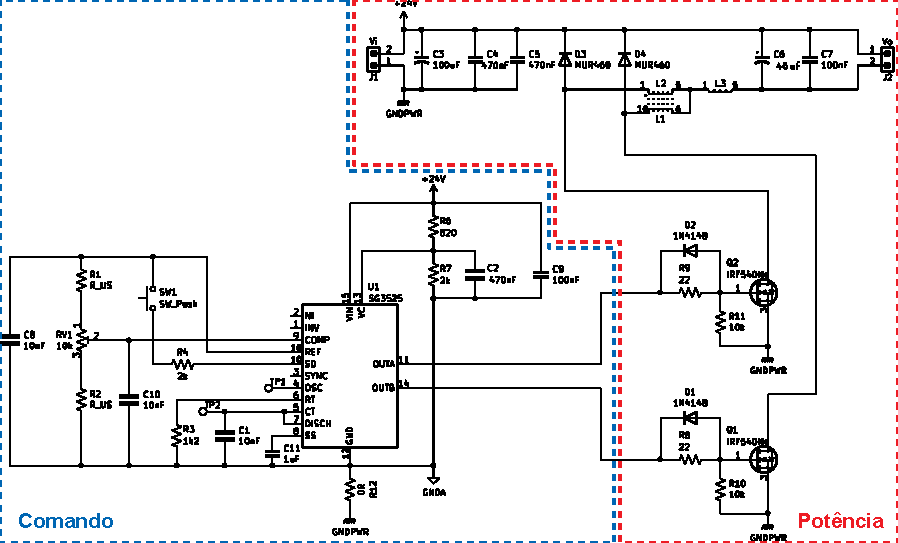
\includegraphics[scale=1]{pdf/layout/Esquematico_CBI_kicad_3.pdf}
        \label{fig:esquematico_cbi}
     	\indentedfont[15.2cm]{Elaboração própria (2021)}
    \end{figure}
    
    Seguido do desenvolvido do esquemático, projetou-se o \textit{layout} da PCB, mostrado na \autoref{fig:layout_cbi}. Durante esse processo, também seguiu-se as boas práticas de desenvolvimento de um \textit{layout} de PCB. 
    
    \begin{figure}[H]
    	\centering
    	\caption{\textit{Layout} desenvolvido do CBI de dois ramos}
    	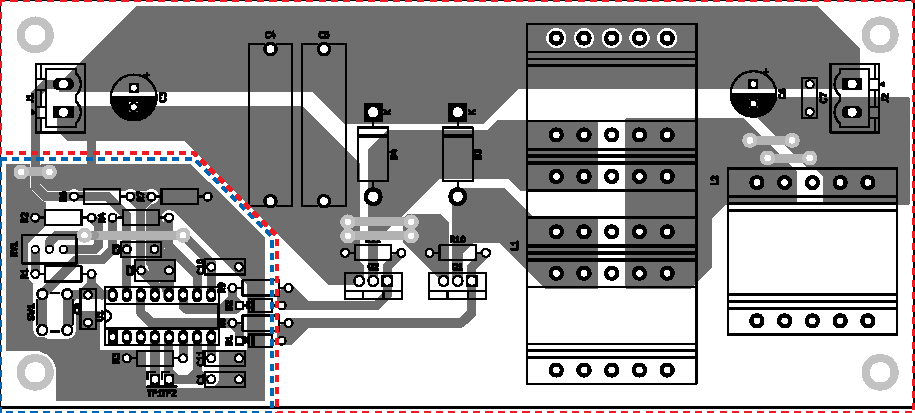
\includegraphics[scale=1]{pdf/layout/layout_CBI4.pdf}
        \label{fig:layout_cbi}
     	\indentedfont[15.5cm]{Elaboração própria (2021)}
    \end{figure}
    
    No desenvolvimento do \textit{layout}, teve-se o cuidado para isolar as referências de comando (azul) e potência (vermelho), como mostrado na \autoref{fig:layout_cbi}, e manter o fluxo de potência em um mesmo sentido, com laços de alta frequência pequenos, como pode ser observado na \autoref{fig:layout_cbi_boas_prat}.
    
    \begin{figure}[H]
    	\centering
    	\caption{Análise do \textit{layout} desenvolvido do CBI de dois ramos}
    	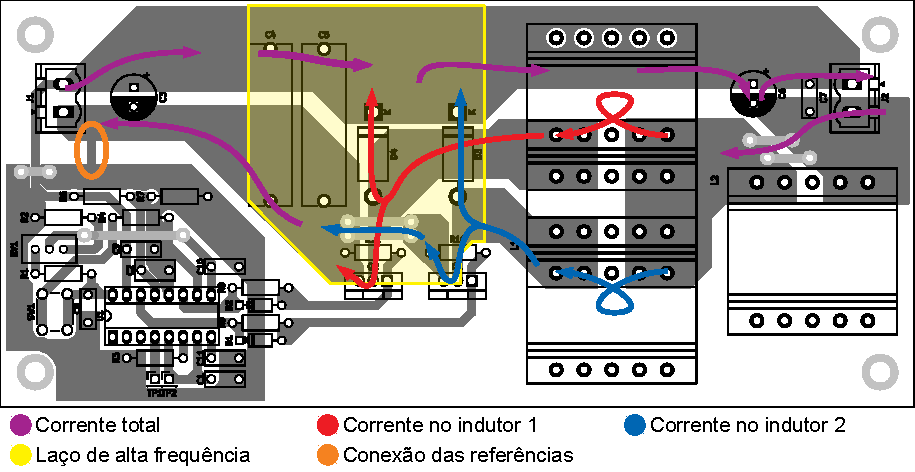
\includegraphics[scale=1]{pdf/layout/layout_CBI3.pdf}
        \label{fig:layout_cbi_boas_prat}
     	\indentedfont[15.5cm]{Elaboração própria (2021)}
    \end{figure}
    
    Finalizada a PCB, se iniciou os testes elétricos do CBI de dois ramos, para que fosse possível a validação do seu correto funcionamento. Nesses testes, foi percebido que, devido à elevada variação da corrente de saída, de aproximadamente \SI{2}{\ampere}, segundo \citeonline{ref:esr_capacitor}, o capacitor utilizado necessitaria de uma ESR máxima de \SI{6}{\milli$\Omega$}, para que assim fosse possível atender as especificações da variação de tensão de saída. Dessa forma, pela disponibilidade e dificuldade para se obter capacitores com ESR tão baixa, foi utilizado em paralelo dois capacitores eletrolítico de baixa resistência série, com valor de capacitância de \SI{470}{\micro\farad}. Assim, a \autoref{fig:esquematico_cbi_1} apresenta, sem o circuito de acionamento, o circuito de potência do conversor utilizado. 
    
    \begin{figure}[H]
    	\centering
    	\caption{Esquemático simplificado utilizado do CBI de dois ramos}
    	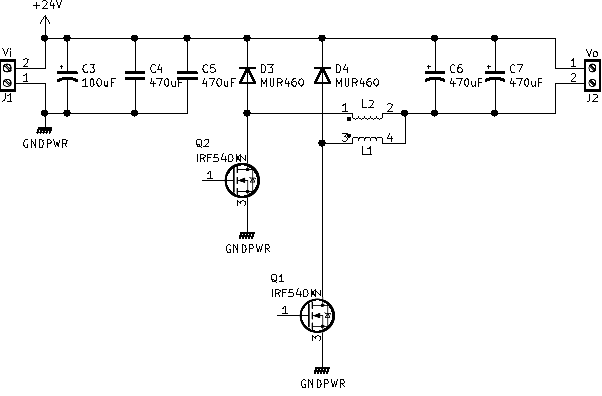
\includegraphics[scale=1.2]{pdf/layout/Esquematico_CBI_simples.pdf}
        \label{fig:esquematico_cbi_1}
     	\indentedfont[12.5cm]{Elaboração própria (2021)}
    \end{figure}
    
    O modelo 3D da placa desenvolvida para o conversor proposto pode ser observado na \autoref{fig:3d_placa_inicial}.
    
    \begin{figure}[H]
    	\centering
    	\caption{Modelo 3D do conversor desenvolvido}
    	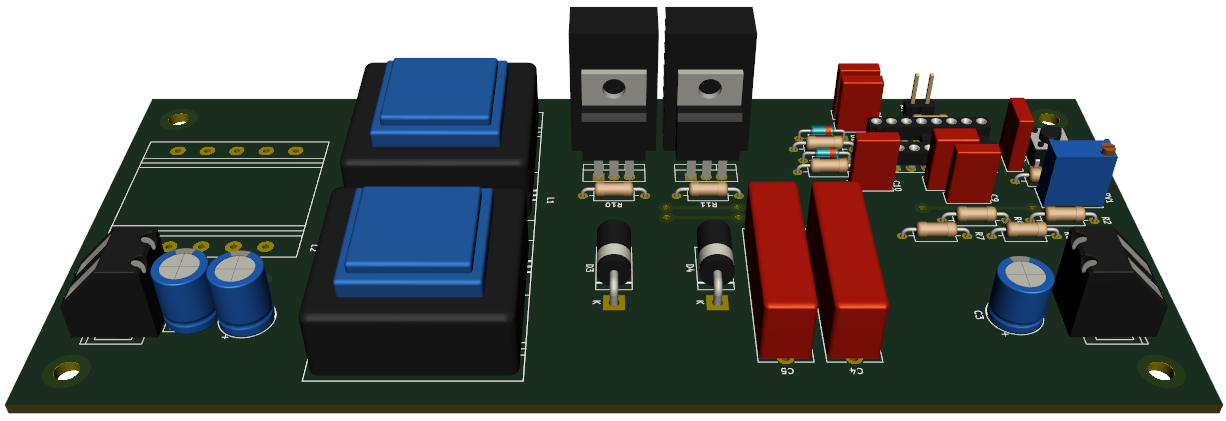
\includegraphics[scale=.35]{pdf/fotos/placa_inicial.png}
        \label{fig:3d_placa_inicial}
     	\indentedfont[15.5cm]{Elaboração própria (2021)}
    \end{figure}
    
    
    %Dessa forma, a \autoref{fig:tensao_dc_cbi} apresenta a tensão de saída do CBI de dois ramos. 
    
    %\begin{figure}[H]
    %	\centering
    %	\caption{Medida em osciloscópio da tensão de saída do CBI de dois ramos}
    %	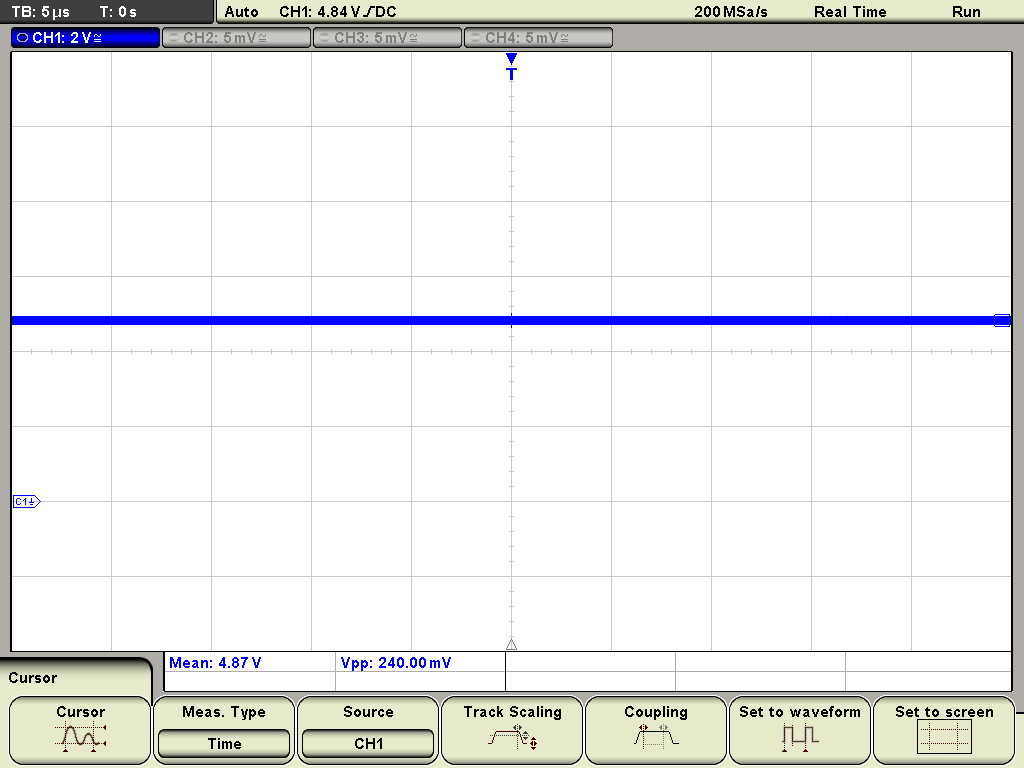
\includegraphics[scale=.4]{pdf/resultados/NEW29.PNG}
    %    \label{fig:tensao_dc_cbi}
    % 	\indentedfont[12.5cm]{Elaboração própria (2021)}
    %\end{figure}
    
    %Após essas alterações, com exceção da variação da tensão de saída que permaneceu em \SI{2}{\%}, como mostrado na \autoref{fig:tensao_ac_cbi}, todos os demais requisitos elétricos estabelecidos para o projeto puderam ser alcançados e validados. Devido à especificação da variação da tensão de saída ser muita pequena, optou-se por mantê-la em \SI{2}{\%}, ao invés de aumentar a capacitância de saída.
    
    %\begin{figure}[H]
    %	\centering
    %	\caption{Medida em osciloscópio da variação da tensão de saída do CBI de dois ramos}
    %	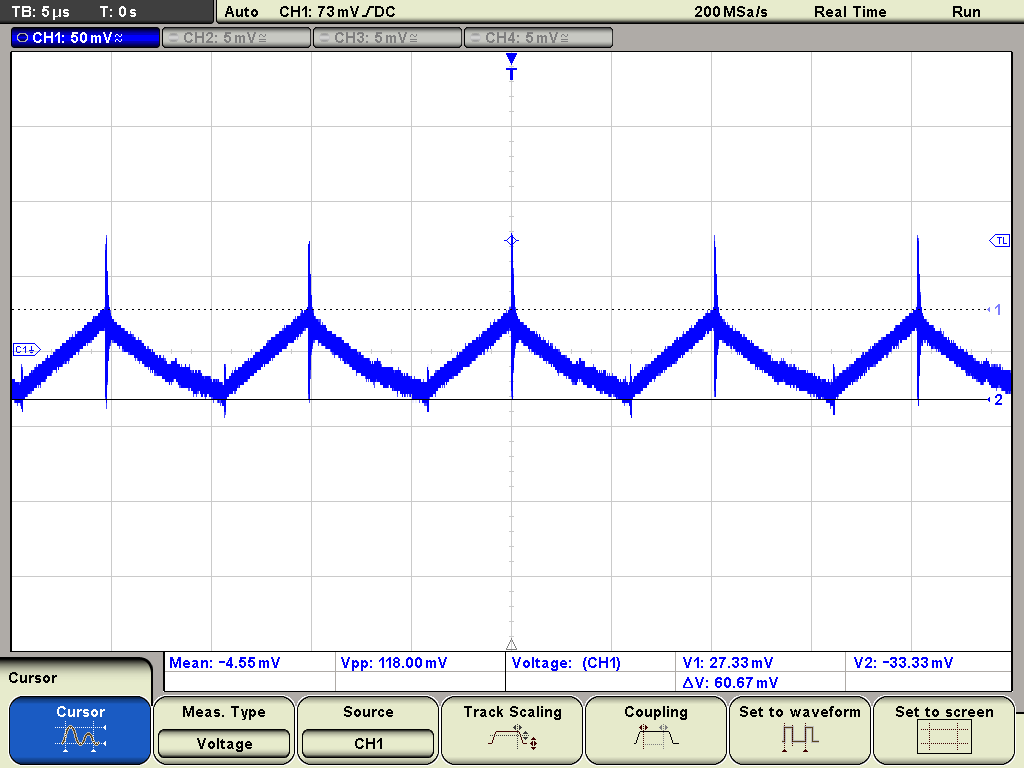
\includegraphics[scale=.4]{pdf/resultados/NEW30.PNG}
    %    \label{fig:tensao_ac_cbi}
    % 	\indentedfont[12.5cm]{Elaboração própria (2021)}
    %\end{figure}
    
    Após essas alterações, com exceção da variação da tensão de saída que permaneceu em \SI{2}{\%}, todos os demais requisitos elétricos estabelecidos para o projeto puderam ser alcançados e validados. Devido à especificação da variação da tensão de saída ser muita pequena, optou-se por mantê-la em \SI{2}{\%}, ao invés de aumentar a capacitância de saída.
    
    %%%%%%%%%%%%%%%%%%%%%%%%%%%%%%%%%%%%%%%%%%%%%%%%%%%%%%%%%%%%%%%%%%%
    \section{Padronização de medidas} \label{cap:result_padrao}
    %%%%%%%%%%%%%%%%%%%%%%%%%%%%%%%%%%%%%%%%%%%%%%%%%%%%%%%%%%%%%%%%%%%
    
    Após a validação elétrica do CBI de dois ramos, para que fosse possível realizar as medidas de EMI de forma mais confiável, sem impactos nos resultados provenientes de fatores alheios as técnicas propostas, foram feitas medições para averiguar a necessidade da padronização da medida.  
    
    A primeira medida realizada foi com relação a influência da posição do cabo na medida de EMI irradiada. Nesse teste, o cabo de alimentação e da carga do produto sob teste (o CBI de dois ramos) foram posicionados de duas formas distintas, cabo descendo de forma paralela até o chão da câmara (Medida 1) e cabo descendo de forma descuidada até o chão da câmara (Medida 2). A \autoref{fig:med_rad_cabo} apresenta os resultados obtidos com a medida. 
    
    \begin{figure}[H]
    	\centering
    	\caption{Espectro de emissão irradiada para o ensaio da influência do posicionamento do cabo de carga e alimentação nas medidas}
    	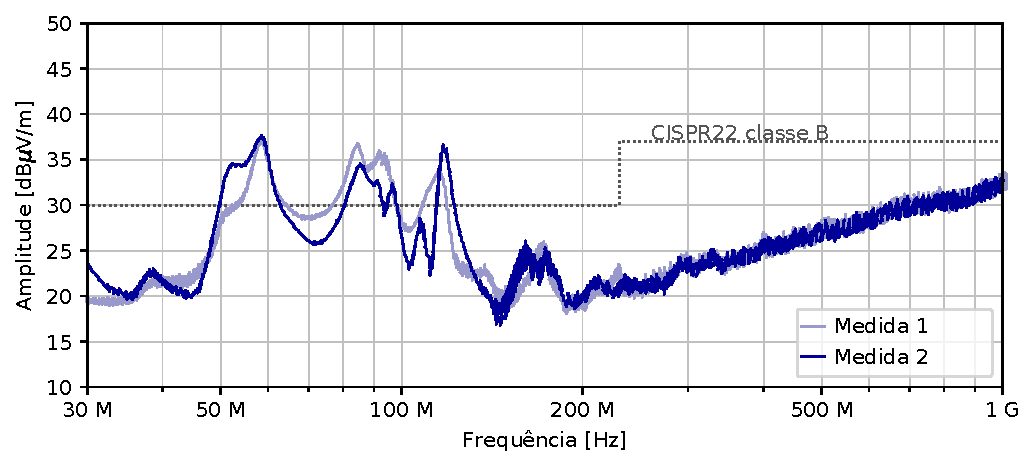
\includegraphics[scale=.9]{pdf/rad/Sem o cuidado com o cabo2.pdf}
    	\label{fig:med_rad_cabo}
     	\indentedfont[15.5cm]{Elaboração própria (2021)}
    \end{figure}
    
    Nota-se pela figura que o posicionamento dos cabos é de grande influência nas medidas. Dessa forma, evitando erros de medida, padronizou-se a posição do cabo como a utilizada na Medida 1.
    
    O segundo teste realizado foi do produto em regime térmico. Esse teste teve como objetivo verificar se haveria uma alteração na medida de EMI conduzida e irradiada do produto em temperatura ambiente e em regime térmico. Porém, após realizado, verificou-se que não havia variações nas medidas, podendo dessa forma realizar os testes futuros sem que houvesse a necessidade de deixar o produto em regime térmico antes de realizar as medidas. 
    
    Por último, após alguns testes, verificou-se a influência da rotação da placa dentro da câmara para um mesmo eixo medido nos testes de EMI irradiada. Nesse teste, percebeu-se que há uma grande variação na medida se os componentes presentes na placa estão voltados para a parede da câmara contendo o absorvedor de ondas electromagnéticas ou a porta da câmara. A \autoref{fig:med_rad_rot_placa} apresenta as medidas obtidas nesse teste para um dos eixos. 
    
    \begin{figure}[H]
    	\centering
    	\caption{Espectro de emissão irradiada para o ensaio da rotação da placa dentro da câmara para um mesmo eixo}
    	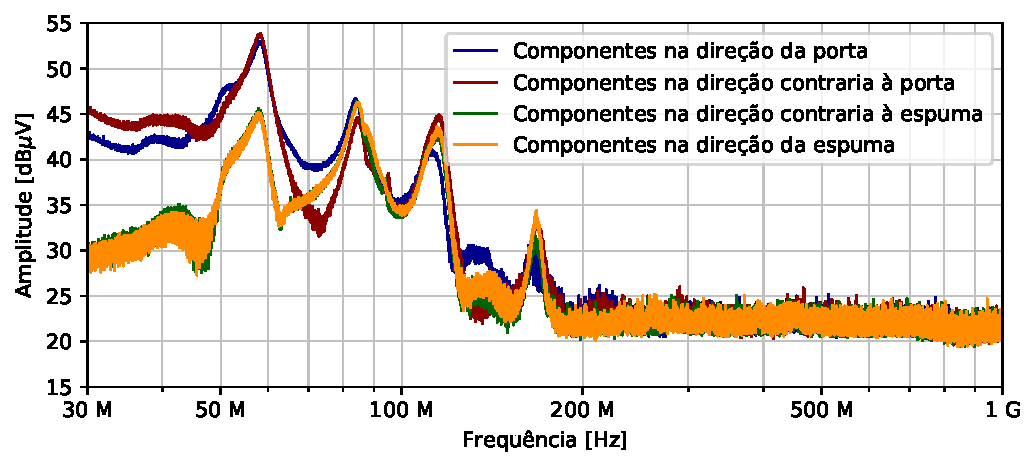
\includegraphics[scale=.9]{pdf/rad/rotacionando.pdf}
    	\label{fig:med_rad_rot_placa}
     	\indentedfont[15.5cm]{Elaboração própria (2021)}
    \end{figure}
    
    Com esse resultado, usou-se como padrão as medidas da placa com a face contendo os componentes voltada para a porta da câmara devido à maior facilidade de posicionamento.
    
    %%%%%%%%%%%%%%%%%%%%%%%%%%%%%%%%%%%%%%%%%%%%%%%%%%%%%%%%%%%%%%%%%%%
    \section{Técnicas de mitigação de EMI} \label{cap:result_tecnicas}
    %%%%%%%%%%%%%%%%%%%%%%%%%%%%%%%%%%%%%%%%%%%%%%%%%%%%%%%%%%%%%%%%%%%
    
    Tendo estabelecido um padrão de medida, pôde-se dar inicio aos testes de emissão conduzida e irradiada. Todos os testes realizados utilizaram como padrão comparativo a medida inicial (do CBI de dois ramos), para que seja possível analisar apenas os impactos gerados pela nova técnica. A \autoref{fig:med_cond_circ_inic} apresenta a medida inicial de EMI conduzida do CBI de dois ramos. 
    
    %Espectro de emissão irradiada para o ensaio d
    \begin{figure}[H]
    	\centering
    	\caption{Ensaio de emissão conduzida do conversor Buck \Interleaved}
    	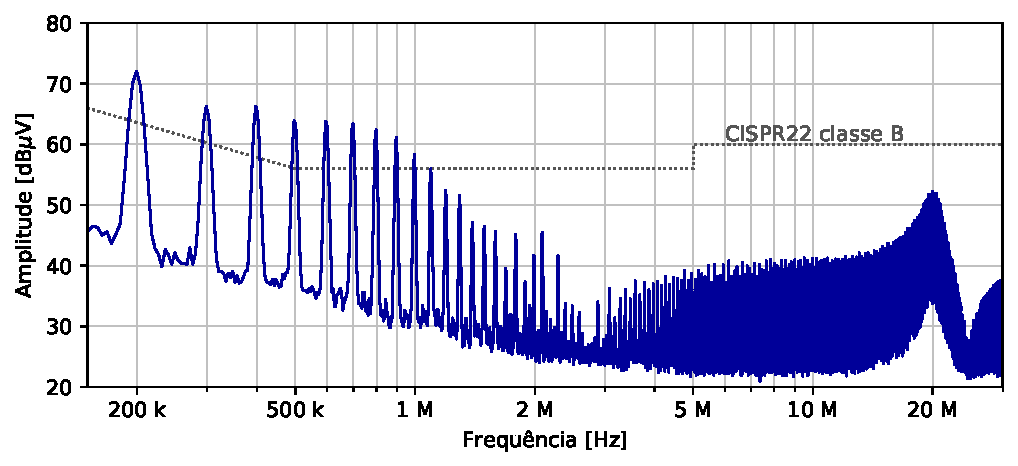
\includegraphics[scale=.9]{pdf/cond/Circuito inicial.pdf}
    	\label{fig:med_cond_circ_inic}
     	\indentedfont[15.5cm]{Elaboração própria (2021)}
    \end{figure}
    
    Nota-se pela figura que o conversor proposto apresenta elevados níveis de ruído conduzido em frequências múltiplas de \SI{100}{\kilo\hertz}. Tal fato se dá devido à haver no circuito dois chaveamentos em uma frequência de \SI{50}{\kilo\hertz} defasados em \SI{180}{\degree}. Ainda, destaca-se que há uma redução progressiva na amplitude dos harmônicos medidos, voltando a crescer após a frequência de \SI{3}{\mega\hertz}, com um pico em torno da frequência de \SI{20}{\mega\hertz}.
    
    Na \autoref{fig:med_rad_circ_inic} temos a medida inicial de EMI irradiada do CBI de dois ramos. 
    
    \begin{figure}[H]
    	\centering
    	\caption{Ensaio de emissão irradiada do conversor Buck \Interleaved}
    	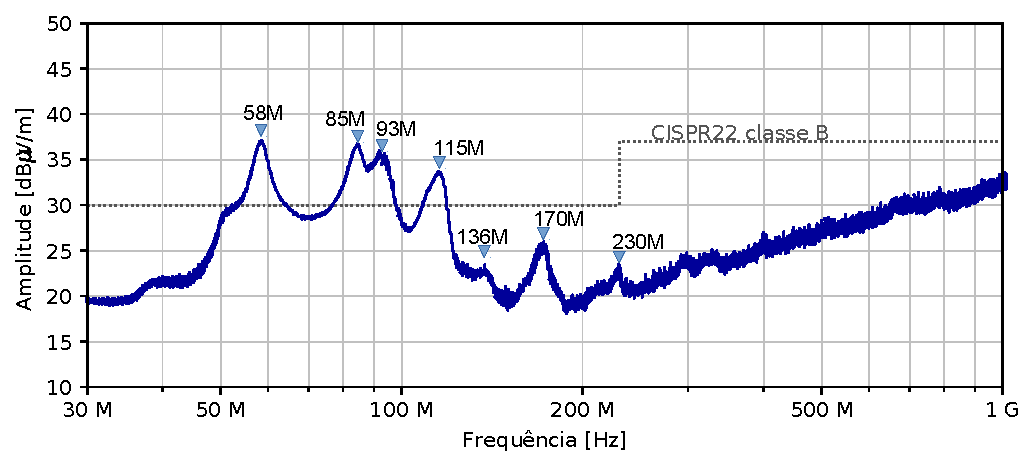
\includegraphics[scale=.9]{pdf/rad/Circuito inicial_2.pdf}
    	\label{fig:med_rad_circ_inic}
     	\indentedfont[15.5cm]{Elaboração própria (2021)}
    \end{figure}
    
    Nessa figura é possível observar alguns picos com amplitudes mais elevadas nas frequência do entorno de \SI{58}{\mega\hertz}, \SI{85}{\mega\hertz}, \SI{93}{\mega\hertz}, \SI{115}{\mega\hertz}, \SI{136}{\mega\hertz}, \SI{170}{\mega\hertz} e \SI{230}{\mega\hertz}, sendo esses picos de maior interesse de redução durante os testes das técnicas.
    
    Com as medidas obtidas, analisando o conversor proposto e a bibliografia, escolheu-se algumas técnicas de mitigação de EMI. As técnicas utilizadas foram apresentadas conforme o ponto de aplicação, sendo elas: o dissipador, o transistor, o indutor e a estrutura do conversor. 
    
    %%%%%%%%%%%%%%%%%%%%%%%%%%%%%%%%%%%%%%%%%%%%%%%%%%%%%%%%%%%%%%%%%%%
    \subsection{Técnicas relacionadas ao elemento dissipador} \label{cap:result_tecnicas_dissip}
    %%%%%%%%%%%%%%%%%%%%%%%%%%%%%%%%%%%%%%%%%%%%%%%%%%%%%%%%%%%%%%%%%%%
    
    A primeira técnica avaliada por esse trabalho, que visa analisar o impacto dos dissipadores nas medidas de emissão conduzida e irradiada, consiste na remoção dos dissipadores presentes nos transistores, representado na \autoref{fig:3d_tecnica_dissipador}. Tal teste foi possível devido aos transistores utilizados na estrutura, sem dissipador, quando em funcionamento, estarem dentro da faixa térmica limite de operação. 
    
    \begin{figure}[H]
    	\centering
    	\caption{Modelo 3D do conversor desenvolvido sem os dissipadores}
    	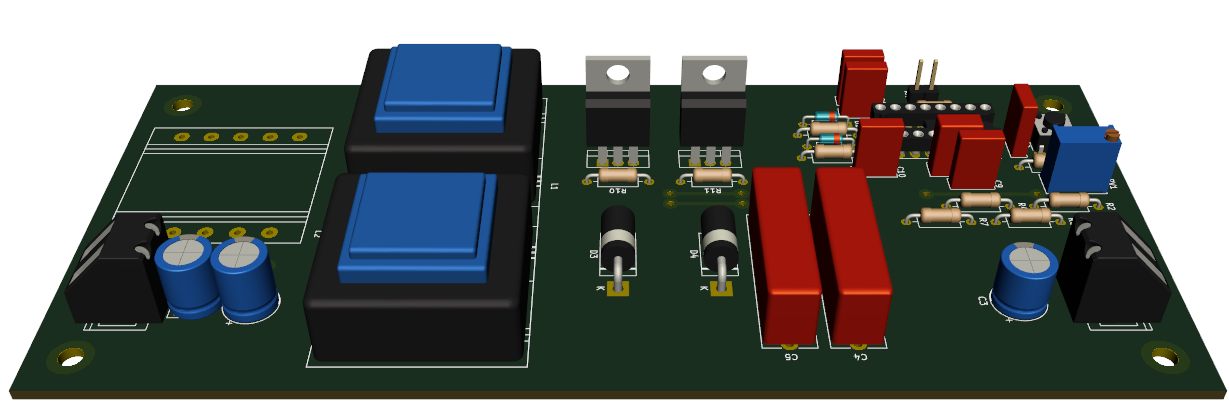
\includegraphics[scale=.35]{pdf/fotos/tecnica_dissipador.png}
        \label{fig:3d_tecnica_dissipador}
     	\indentedfont[15.5cm]{Elaboração própria (2021)}
    \end{figure}
    
    A \autoref{fig:med_cond_remv_dissip} apresenta um comparativo da emissão conduzida entre os resultados obtidos ao ser removido os dissipadores conectados aos transistores e a medida de referência (com os dissipadores conectados aos transistores). 
    
    \begin{figure}[H]
    	\centering
    	\caption{Comparação dos resultados do ensaio de emissão conduzida para o circuito sem os dissipadores e com os dissipadores conectados aos transistores}
    	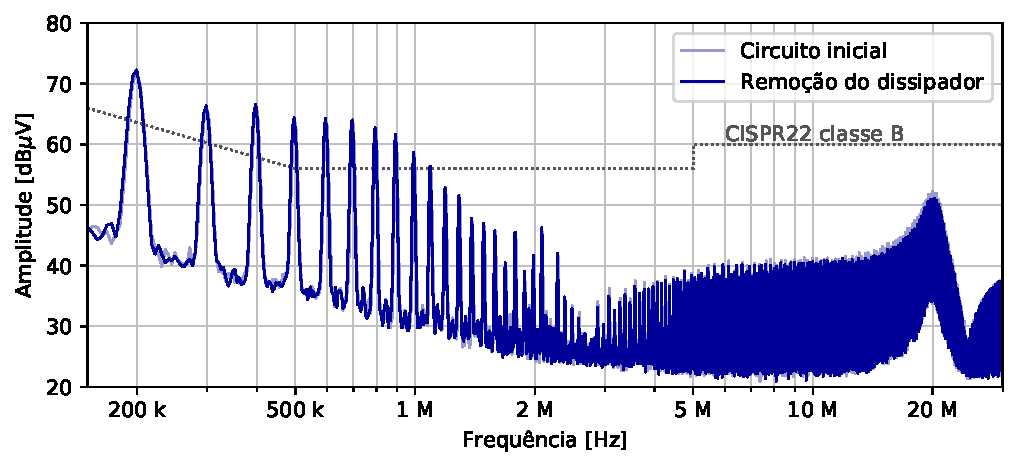
\includegraphics[scale=.9]{pdf/cond/Remoção do dissipador.pdf}
    	\label{fig:med_cond_remv_dissip}
     	\indentedfont[15.5cm]{Elaboração própria (2021)}
    \end{figure}
    
    Nota-se pela figura que não houve grandes mudanças nos resultados da emissão conduzida ao serem removidos os dissipadores, como já esperado, devido aos seus impactos serem principalmente na emissão irradiada. Dessa forma, a \autoref{fig:med_rad_remv_dissip} apresenta o comparativo da emissão irradiada entre os resultados obtidos ao serem removidos os dissipadores conectados aos transistores e a medida de referência. 
    
    \begin{figure}[H]
    	\centering
    	\caption{Comparação dos resultados do ensaio de emissão irradiada para o circuito sem os dissipadores e com os dissipadores conectados aos transistores}
    	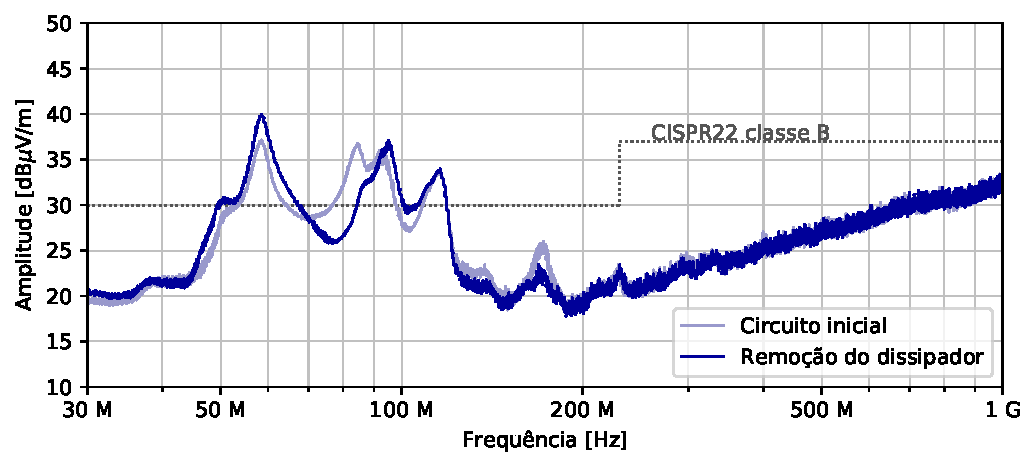
\includegraphics[scale=.9]{pdf/rad/Remoção do dissipador.pdf}
    	\label{fig:med_rad_remv_dissip}
     	\indentedfont[15.5cm]{Elaboração própria (2021)}
    \end{figure}
    
    Pela figura, percebe-se uma pequena alteração dos resultados obtidos. No entorno das frequências de \SI{58}{\mega\hertz} e \SI{93}{\mega\hertz} houve um pequeno acréscimo na emissão irradiada, enquanto nas frequências de \SI{85}{\mega\hertz} e \SI{170}{\mega\hertz} se obteve uma redução. Dessa forma, essa técnica não apresentou grandes benefícios para a redução das emissões. 
    
    Outra medida realizada, relacionada aos dissipadores, foi a conexão do dissipador a referência utilizando um capacitor cerâmico $\subx{C}{D}$, conforme \autoref{fig:esquematico_cbi_2}. O capacitor foi necessário devido ao dissipador não estar isolado e, portanto, conectado diretamente ao dreno do transistor. Nesta técnica, busca-se criar um caminho de menor impedância para os harmônicos gerados, evitado que o mesmo seja irradiado pelo dissipador. 
    
    \begin{figure}[H]
    	\centering
    	\caption{Esquemático simplificado do CBI de dois ramos com a conexão do dissipador a referência do circuito}
    	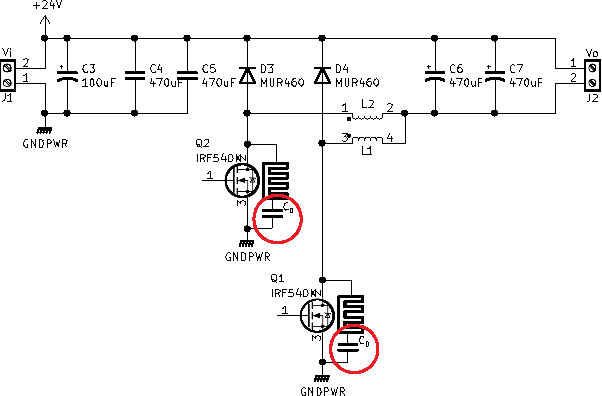
\includegraphics[scale=1.2]{pdf/layout/Esquematico_CBI_dissipador2.pdf}
        \label{fig:esquematico_cbi_2}
     	\indentedfont[12.5cm]{Elaboração própria (2021)}
    \end{figure}
    
    
    O modelo 3D da técnica aplicada no conversor pode ser observada na \autoref{fig:3d_tecnica_capacitor}.
    
    \begin{figure}[H]
    	\centering
    	\caption{Modelo 3D do conversor desenvolvido com capacitores conectados aos dissipadores}
    	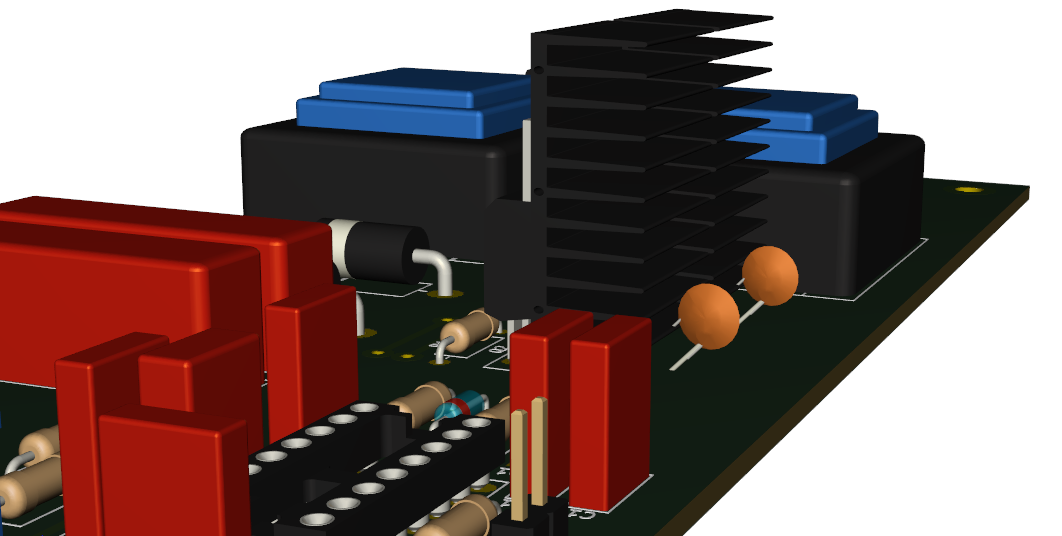
\includegraphics[scale=.35]{pdf/fotos/tecnica_capacitor.png}
        \label{fig:3d_tecnica_capacitor}
     	\indentedfont[15.5cm]{Elaboração própria (2021)}
    \end{figure}
    
    Para esse ensaio, foram arbitrados dois capacitores de diferentes valores, \SI{1}{\nano\farad} e \SI{100}{\nano\farad}, para que fosse possível verificar os impactos gerados pelos valores escolhidos. A \autoref{fig:med_cond_cap1n_dissip} apresenta um comparativo dos resultados obtidos do ensaio de emissão conduzida para o circuito com os dissipadores desconectados e conectados à referência via capacitor de \SI{1}{\nano\farad}.
    
    \begin{figure}[H]
    	\centering
    	\caption{Comparação dos resultados do ensaio de emissão conduzida para o circuito com os dissipadores desconectados e conectados à referência via capacitor de \SI{1}{\nano\farad}}
    	\includegraphics[scale=.9]{pdf/cond/Conectar o dissipador a referência (Capacitor de 1nF).pdf}
    	\label{fig:med_cond_cap1n_dissip}
     	\indentedfont[15.5cm]{Elaboração própria (2021)}
    \end{figure}
    
    Percebe-se que o uso do capacitor, diferentemente da remoção dos dissipadores, impactou na emissão conduzida do ruído. É possível observar na medida que, após a alteração, os harmônicos múltiplos de \SI{50}{\kilo\hertz} estão com maior amplitude do que na medida inicial. Ainda, no entorno da frequência de \SI{20}{\mega\hertz} é perceptível um aumento ainda mais acentuado dos harmônicos. 
    
    A medida de emissão irradiada desse teste, para o circuito com os dissipadores conectados à referência via capacitor de \SI{1}{\nano\farad}, pode ser observado na \autoref{fig:med_rad_cap1n_dissip}. 
    
    \begin{figure}[H]
    	\centering
    	\caption{Comparação dos resultados do ensaio de emissão irradiada para o circuito com os dissipadores desconectados e conectados à referência via capacitor de \SI{1}{\nano\farad}}
    	\includegraphics[scale=.9]{pdf/rad/Conectar o dissipador a referência (Capacitor de 1nF).pdf}
    	\label{fig:med_rad_cap1n_dissip}
     	\indentedfont[15.5cm]{Elaboração própria (2021)}
    \end{figure}
    
    Nessa figura, observa-se que houve grandes reduções em dois principais picos da emissão irradiada nas frequências de \SI{58}{\mega\hertz} e \SI{115}{\mega\hertz}. Ainda, destaca-se a redução de amplitude em frequências inferiores a \SI{70}{\mega\hertz}. Porém, têm-se uma elevação na amplitude em outras frequências. 
    
    Essa técnica, utilizando um capacitor de \SI{1}{\nano\farad}, apesar de apresentar melhoras em determinadas frequências na emissão irradiada, apresentou pioras em outras frequências, inclusive na emissão conduzida. A \autoref{fig:med_cond_cap100n_dissip} apresenta a mesma técnica, porém utilizando um capacitor de \SI{100}{\nano\farad}, para a emissão conduzida.
    
    \begin{figure}[H]
    	\centering
    	\caption{Comparação dos resultados do ensaio de emissão conduzida para o circuito com os dissipadores desconectados e conectados a referência via capacitor de \SI{100}{\nano\farad}}
    	\includegraphics[scale=.9]{pdf/cond/Conectar o dissipador a referência (Capacitor de 100nF).pdf}
    	\label{fig:med_cond_cap100n_dissip}
     	\indentedfont[15.5cm]{Elaboração própria (2021)}
    \end{figure}
    
    Nota-se que, diferente do resultado obtido para um capacitor de \SI{1}{\nano\farad}, ao utilizar um capacitor cerâmico de \SI{100}{\nano\farad}, há uma redução da amplitude da emissão conduzida no entorno da frequência de \SI{20}{\mega\hertz}. 
    
    O comparativo da emissão irradiada desse teste, para o circuito com os dissipadores conectados e desconectados da referência pode ser observado na \autoref{fig:med_rad_cap100n_dissip}.
    
    \begin{figure}[H]
    	\centering
    	\caption{Comparação dos resultados do ensaio de emissão irradiada para o circuito com os dissipadores desconectados e conectados a referência via capacitor de \SI{100}{\nano\farad}}
    	\includegraphics[scale=.9]{pdf/rad/Conectar o dissipador a referência (Capacitor de 100nF).pdf}
    	\label{fig:med_rad_cap100n_dissip}
     	\indentedfont[15.5cm]{Elaboração própria (2021)}
    \end{figure}
    
    Na figura, pode-se verificar que o uso de um capacitor de \SI{100}{\nano\farad} gerou uma grande redução nos níveis de emissão irradiada para quase todas as frequências, com exceção de poucas frequências, como o caso do entorno de \SI{170}{\mega\hertz}. Assim, percebe-se que, para o conversor proposto, o uso da técnica de aterramento do dissipador apresenta melhores resultados, se comparado a remoção do dissipador. Porém, a escolha do valor da capacitância é de grande impacto nos resultados, como pode-se observar na \autoref{fig:med_cond_cap1n_cap100n_dissip}, que apresenta o comparativos dos resultados obtidos da emissão conduzida.
    
    \begin{figure}[H]
    	\centering
    	\caption{Comparação dos resultados do ensaio de emissão conduzida para o circuito com os dissipadores conectados a referência via capacitor de \SI{1}{\nano\farad} e \SI{100}{\nano\farad}}
    	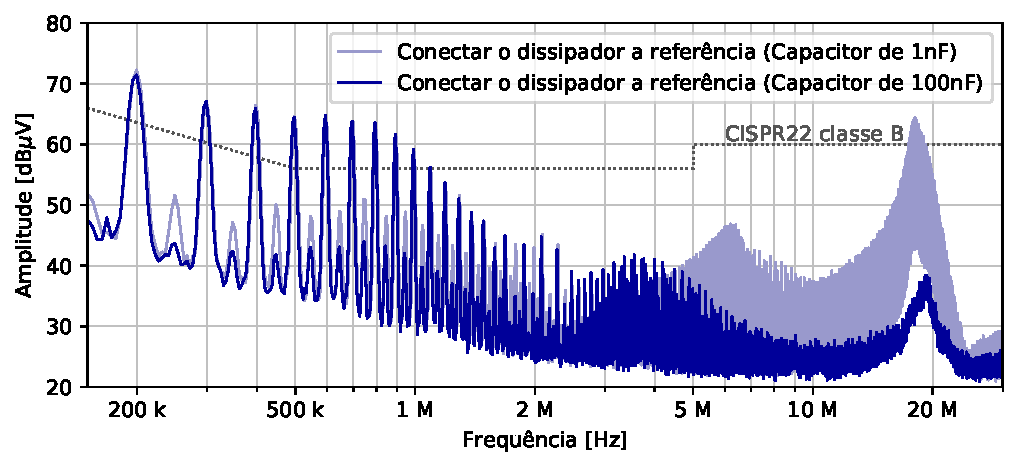
\includegraphics[scale=.85]{pdf/cond/cond-Conectar o dissipador a referência (Capacitor de 1nF)-Conectar o dissipador a referência (Capacitor de 100nF).pdf}
    	\label{fig:med_cond_cap1n_cap100n_dissip}
     	\indentedfont[15.5cm]{Elaboração própria (2021)}
    \end{figure}
    
    O mesmo comprativo, para a emissão irradiada, pode ser observada na \autoref{fig:med_rad_cap1n_cap100n_dissip}.
    
    \begin{figure}[H]
    	\centering
    	\caption{Comparação dos resultados do ensaio de emissão irradiada para o circuito com os dissipadores conectados a referência via capacitor de \SI{1}{\nano\farad} e \SI{100}{\nano\farad}}
    	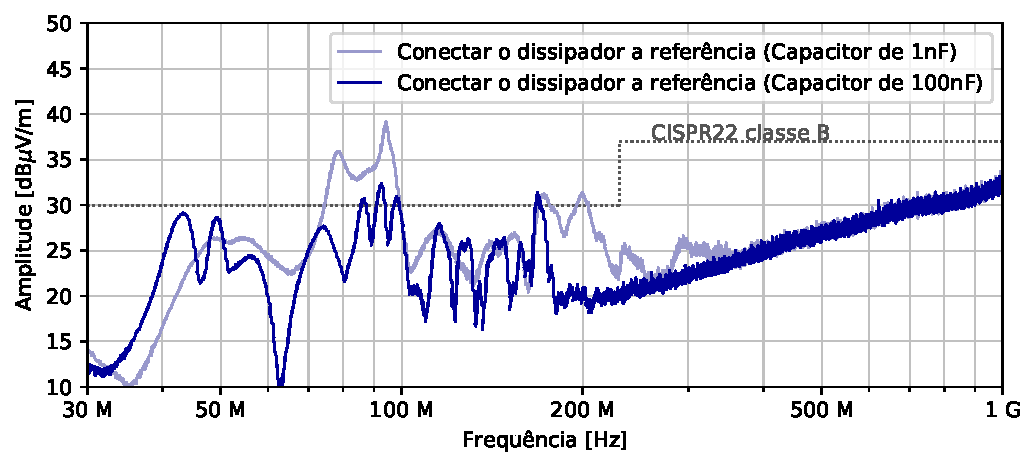
\includegraphics[scale=.85]{pdf/rad/Conectar o dissipador a referência (Capacitor de 1nF)-Conectar o dissipador a referência (Capacitor de 100nF).pdf}
    	\label{fig:med_rad_cap1n_cap100n_dissip}
     	\indentedfont[15.5cm]{Elaboração própria (2021)}
    \end{figure}

    % FALAR MAIS ALGUMA COISA??

    %%%%%%%%%%%%%%%%%%%%%%%%%%%%%%%%%%%%%%%%%%%%%%%%%%%%%%%%%%%%%%%%%%%
    \subsection{Técnicas relacionadas ao elemento transistor} \label{cap:result_tecnicas_chaveam}
    %%%%%%%%%%%%%%%%%%%%%%%%%%%%%%%%%%%%%%%%%%%%%%%%%%%%%%%%%%%%%%%%%%%
    
    Outra técnica avaliada por esse trabalho, relacionada ao chaveamento do transistor, consiste no aumento do tempo de subida do sinal de dreno. Para esse teste, foi feita uma alteração nos resistores R8 e R9, conforme \autoref{fig:esquematico_cbi_3}, que possuíam valores iniciais de \SI{22}{$\Omega$} (com tempo de subida $\subx{t}{r}$ medido em osciloscópio de \SI{138}{\nano\second}) para um valor de \SI{62}{$\Omega$} (com tempo de subida $\subx{t}{r}$ medido em osciloscópio de \SI{255}{\nano\second}). 
    
    \begin{figure}[H]
    	\centering
    	\caption{Esquemático simplificado do CBI de dois ramos com a alteração nos valores dos resistores R8 e R9}
    	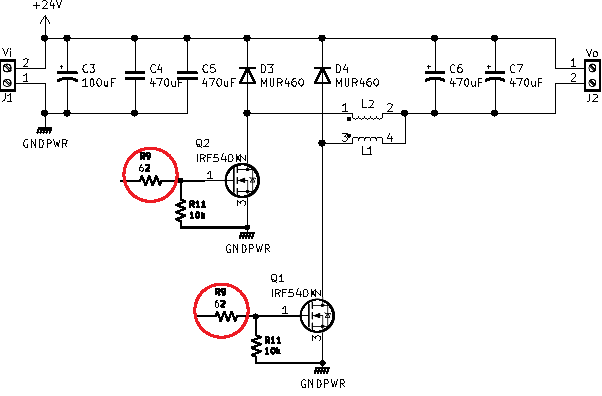
\includegraphics[scale=1.2]{pdf/layout/Esquematico_CBI_tr.pdf}
        \label{fig:esquematico_cbi_3}
     	\indentedfont[12.5cm]{Elaboração própria (2021)}
    \end{figure}
    
    Assim, a \autoref{fig:med_cond_temp_sub} apresenta um comparativo da emissão conduzida entre os resultados obtidos para o circuito inicial ($\subx{t}{r}$ de \SI{138}{\nano\second}) e circuito após alteração dos resistores ($\subx{t}{r}$ de \SI{255}{\nano\second}). 
    
    \begin{figure}[H]
    	\centering 
    	\caption{Comparação dos resultados do ensaio de emissão conduzida para um tempo de subida do sinal no dreno do transistor de \SI{138}{\nano\second} e \SI{255}{\nano\second}}
    	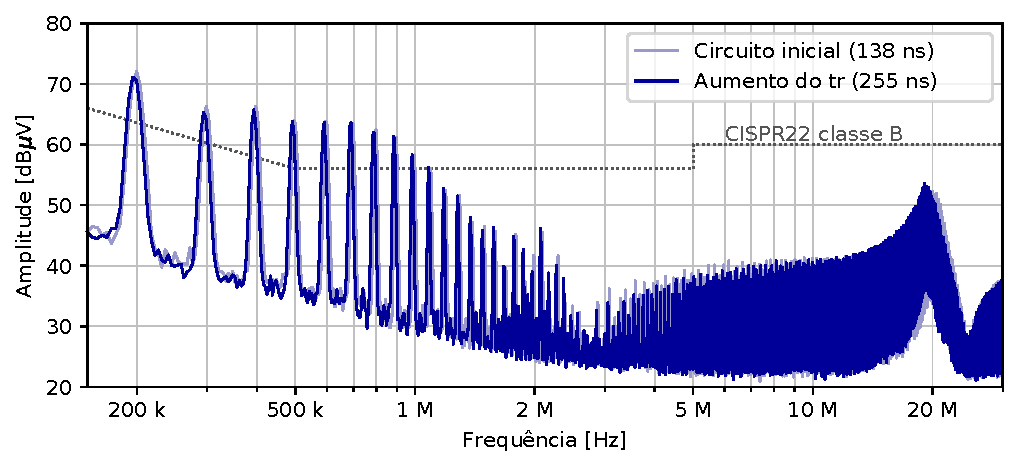
\includegraphics[scale=.9]{pdf/cond/Aumento do tr do transistor2.pdf}
    	\label{fig:med_cond_temp_sub}
     	\indentedfont[15.5cm]{Elaboração própria (2021)}
    \end{figure}
    
    Percebe-se pela figura que a alteração desse tempo de subida não acarretou em grandes alterações nas medidas de emissão conduzida. Na \autoref{fig:med_rad_temp_sub} é possível observar o comparativo da emissão irradiada para o mesmo teste.  
    
    \begin{figure}[H]
    	\centering
    	\caption{Comparação dos resultados do ensaio de emissão irradiada para um tempo de subida do sinal no dreno do transistor de \SI{138}{\nano\second} e \SI{255}{\nano\second}}
    	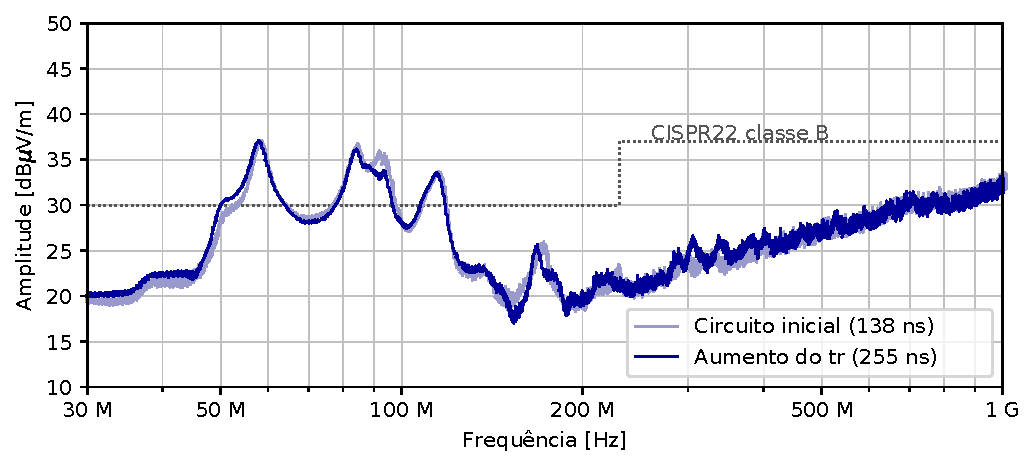
\includegraphics[scale=.9]{pdf/rad/Aumento do tr do transistor2.pdf}
    	\label{fig:med_rad_temp_sub}
     	\indentedfont[15.5cm]{Elaboração própria (2021)}
    \end{figure}
    
    Na emissão irradiada também não houve grandes impactos gerados pela técnica. Esse resultado é devido ao tempo de subida no dreno já ser grande (proveniente do resistor de \SI{22}{$\Omega$}) e assim, esse aumento no tempo de subida, não surtiu efeito para as emissões. 
    
    Ainda relacionado ao dreno do transistor, outra técnica empregada no circuito foi o uso de um núcleo de ferrite \textit{bead} nos terminais de dreno do transistor, como mostrado na \autoref{fig:esquematico_cbi_4}. 
    
    \begin{figure}[H]
    	\centering
    	\caption{Esquemático simplificado do CBI de dois ramos com um núcleo de ferrite no terminal de dreno dos transistores}
    	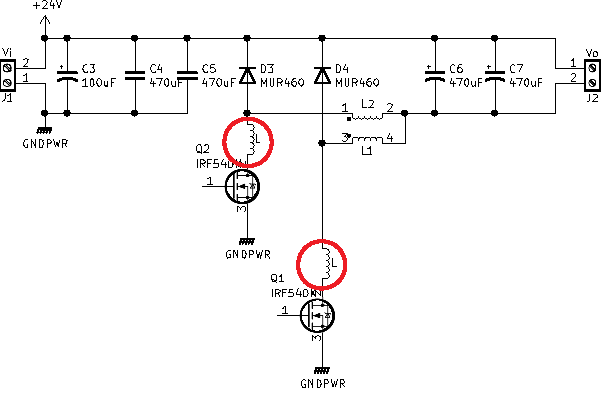
\includegraphics[scale=1.2]{pdf/layout/Esquematico_CBI_bead.pdf}
        \label{fig:esquematico_cbi_4}
     	\indentedfont[12.5cm]{Elaboração própria (2021)}
    \end{figure}
    
    A \autoref{fig:3d_tecnica_choke} apresenta um modelo 3D da técnica aplicada ao conversor.
    
    \begin{figure}[H]
    	\centering
    	\caption{Modelo 3D do conversor desenvolvido com um núcleo de ferrite no terminal de dreno dos transistores}
    	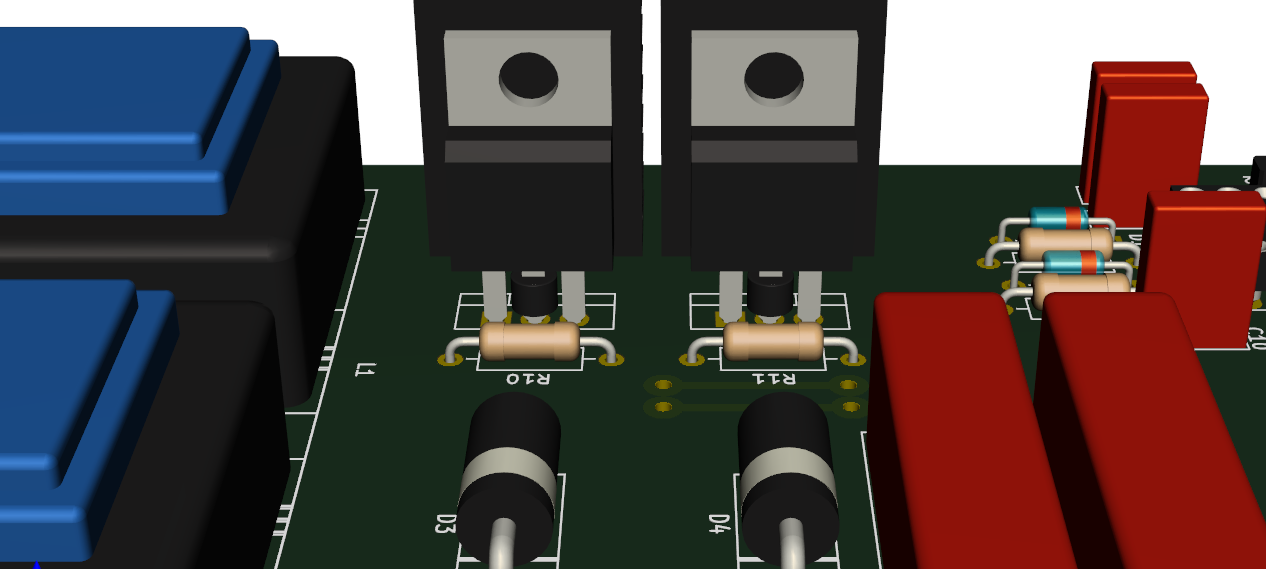
\includegraphics[scale=.35]{pdf/fotos/tecnica_choke2.png}
        \label{fig:3d_tecnica_choke}
     	\indentedfont[15.5cm]{Elaboração própria (2021)}
    \end{figure}
    
    Esta técnica busca confinar no transistor os harmônicos gerados por ele. A \autoref{fig:med_cond_choke} apresenta o comparativo da emissão conduzida entre os resultados obtidos para o circuito inicial (sem o núcleo de ferrite) e o circuito após inserção do núcleo de ferrite \textit{bead}. 
    
    \begin{figure}[H]
    	\centering 
    	\caption{Comparação dos resultados do ensaio de emissão conduzida para o circuito com e sem um núcleo de ferrite nos terminais de dreno dos transistores}
    	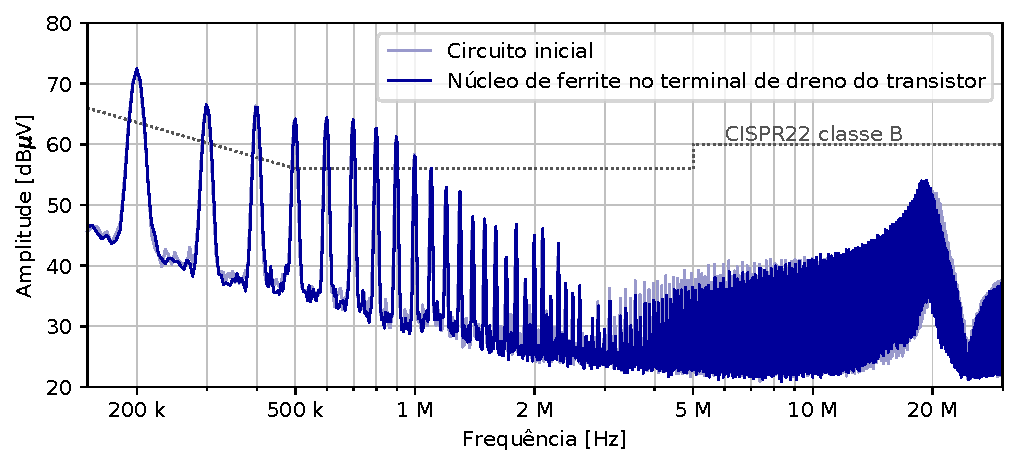
\includegraphics[scale=.9]{pdf/cond/Choke bead no terminal de dreno do transistor.pdf}
    	\label{fig:med_cond_choke}
     	\indentedfont[15.5cm]{Elaboração própria (2021)}
    \end{figure}
    
    Nessa técnica, para a emissão conduzida, também não houve grandes alterações nos resultados. Porém, para a emissão irradiada, algumas mudanças podem ser observadas nas medidas, como na \autoref{fig:med_rad_temp_sub}.  
    
    \begin{figure}[H]
    	\centering
    	\caption{Comparação dos resultados do ensaio de emissão irradiada para o circuito com e sem um núcleo de ferrite nos terminais de dreno dos transistores}
    	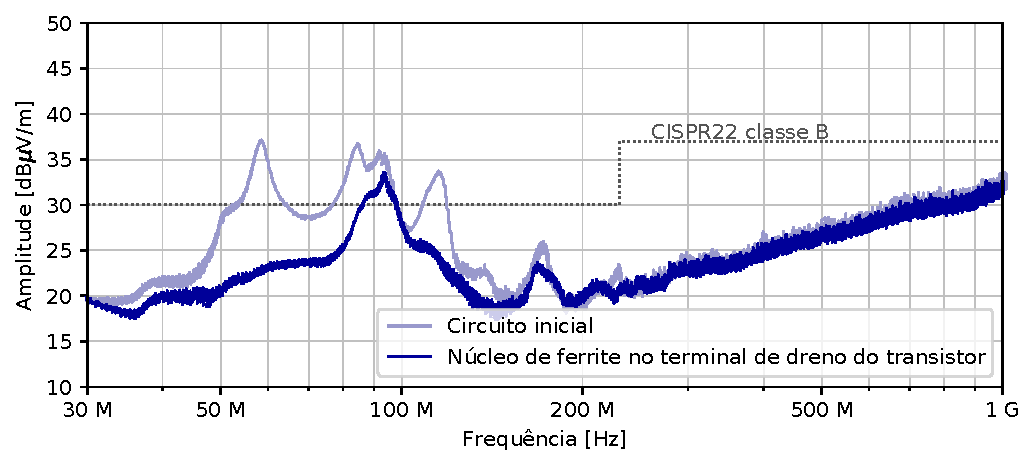
\includegraphics[scale=.9]{pdf/rad/Choke bead no terminal de dreno do transistor.pdf}
    	\label{fig:med_rad_choke}
     	\indentedfont[15.5cm]{Elaboração própria (2021)}
    \end{figure}
    
    Essa técnica mostrou grande eficácia na redução do ruído irradiado, ao contrário da emissão conduzida. Como pode-se observar, a técnica apresentou redução em uma larga faixa de frequência (entre \SI{30}{\mega\hertz} e \SI{200}{\mega\hertz}), com apenas dois picos próximos dos valores iniciais medidos (\SI{93}{\mega\hertz} e \SI{170}{\mega\hertz}).
    
    %%%%%%%%%%%%%%%%%%%%%%%%%%%%%%%%%%%%%%%%%%%%%%%%%%%%%%%%%%%%%%%%%%%
    \subsection{Técnica relacionada ao elemento indutor} \label{cap:result_tecnicas_indut}
    %%%%%%%%%%%%%%%%%%%%%%%%%%%%%%%%%%%%%%%%%%%%%%%%%%%%%%%%%%%%%%%%%%%
    
    Com relação aos indutores, buscando reduzir o acoplamento entre eles, utilizou-se como técnica o reposicionamento de um deles, o rotacionando. Na \autoref{fig:foto_cbi_1} é possível observar a placa inicialmente produzida, com os indutores circulados em vermelho. 
    
    \begin{figure}[H]
    	\centering
    	\caption{Posicionamento dos indutores no circuito inicial}
    	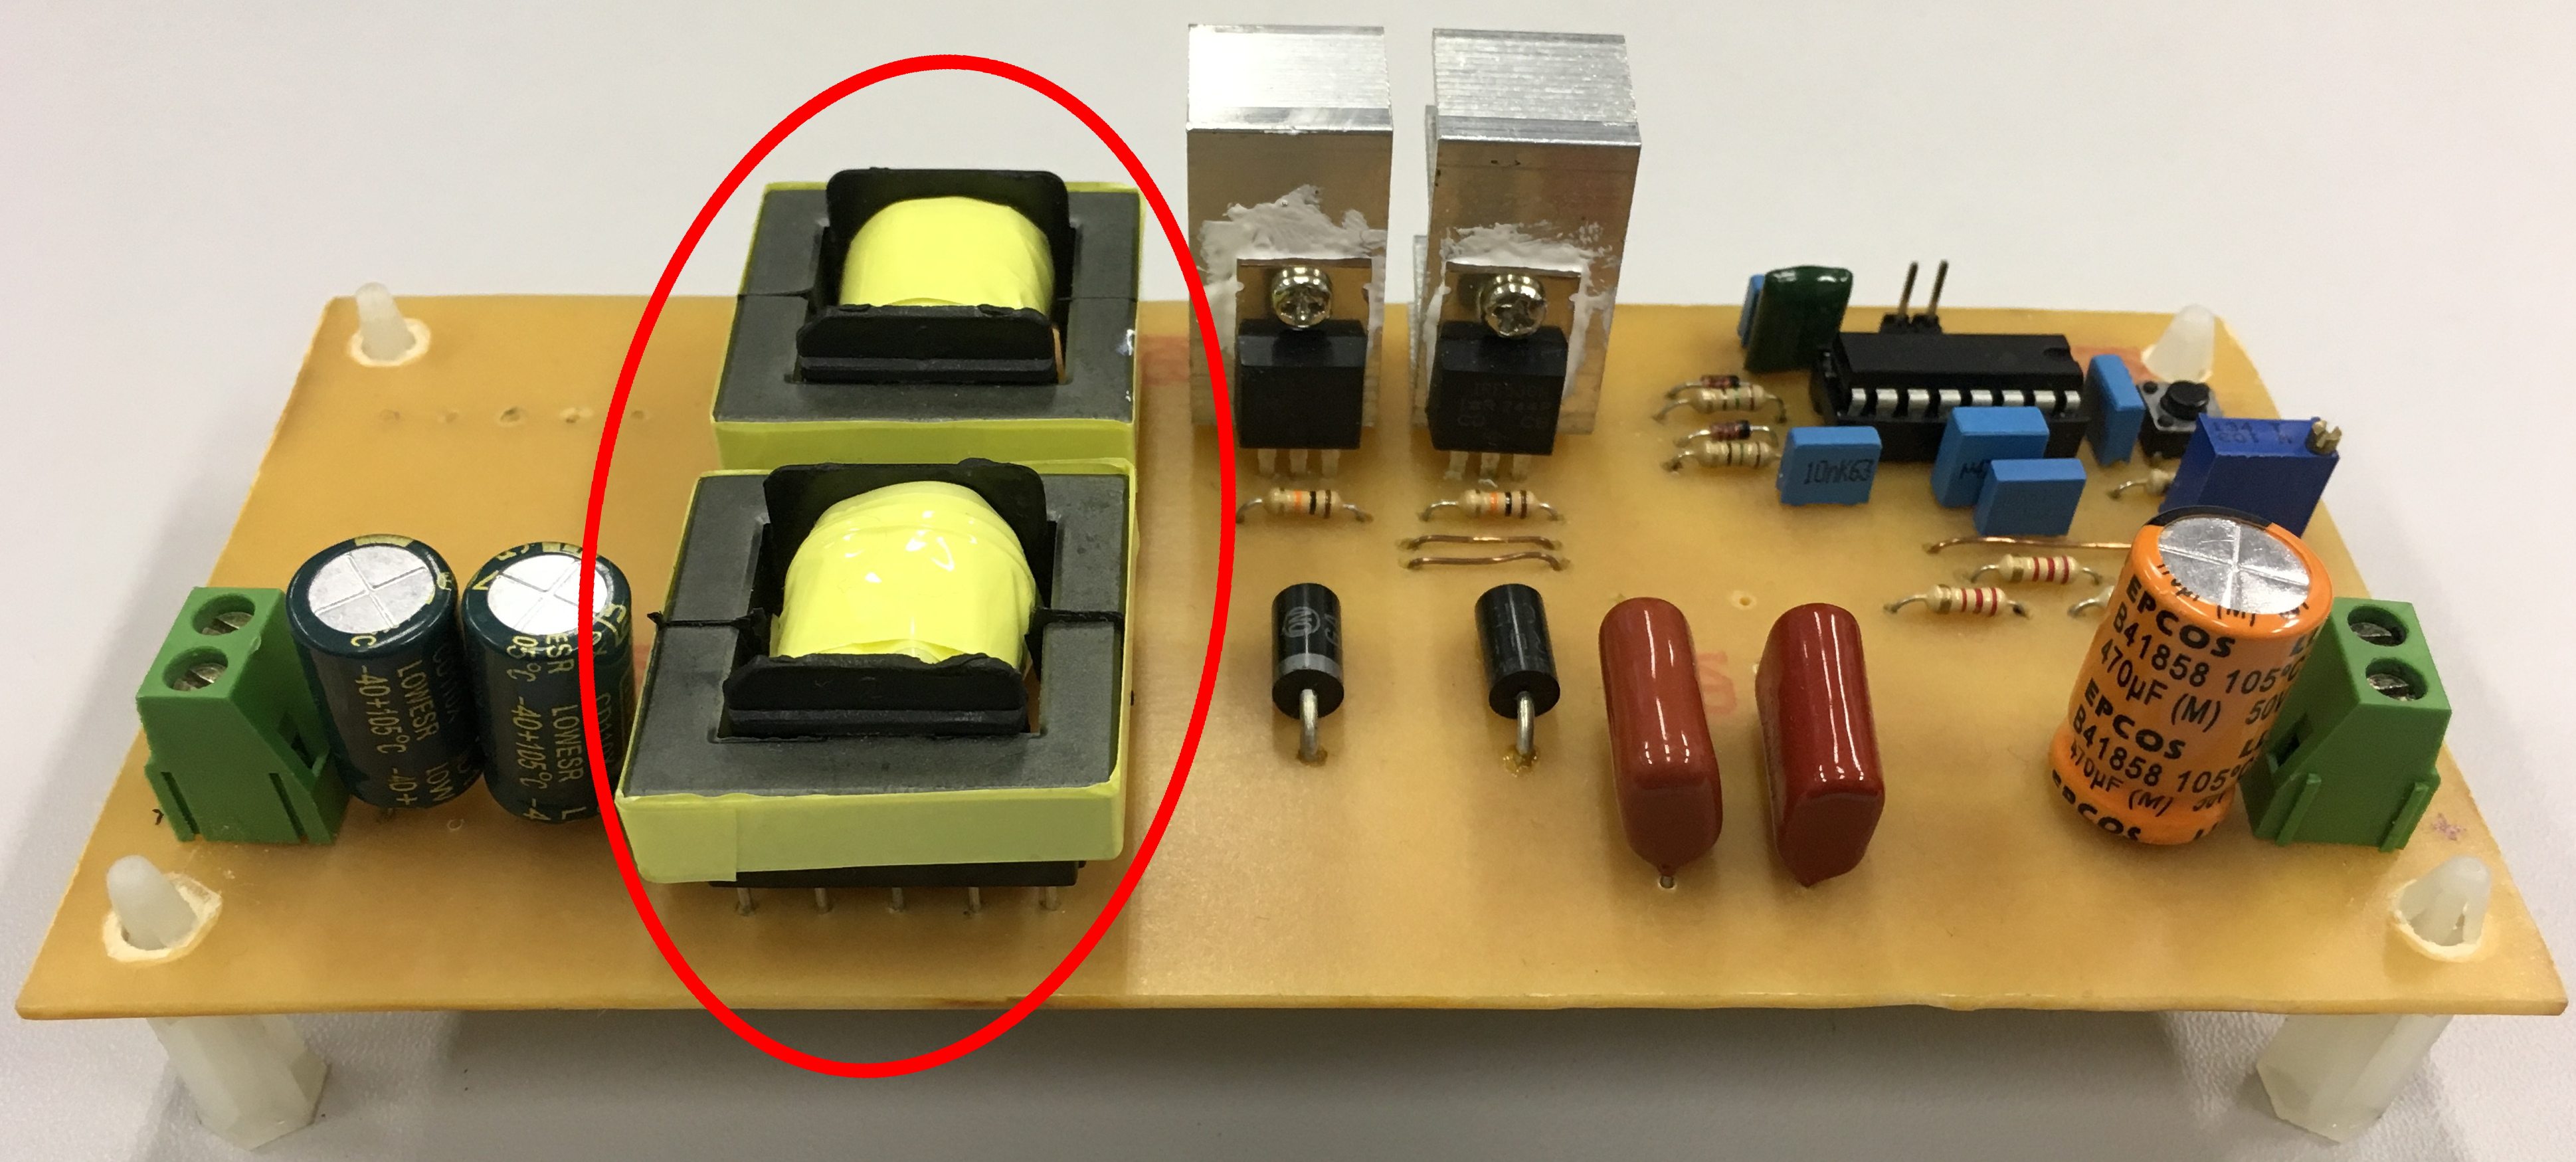
\includegraphics[scale=.1]{pdf/fotos/placa_vista_lateral_sel.jpg}
        \label{fig:foto_cbi_1}
     	\indentedfont[14cm]{Elaboração própria (2021)}
    \end{figure}
    
    Percebe-se pela figura, que ambos os indutores estão posicionados paralelamente e com seus fluxos na mesma direção, como demonstrado na \autoref{fig:foto_cbi_2}.
    
    \begin{figure}[H]
    	\centering
    	\caption{Representação do fluxo dos indutores no circuito inicial}
    	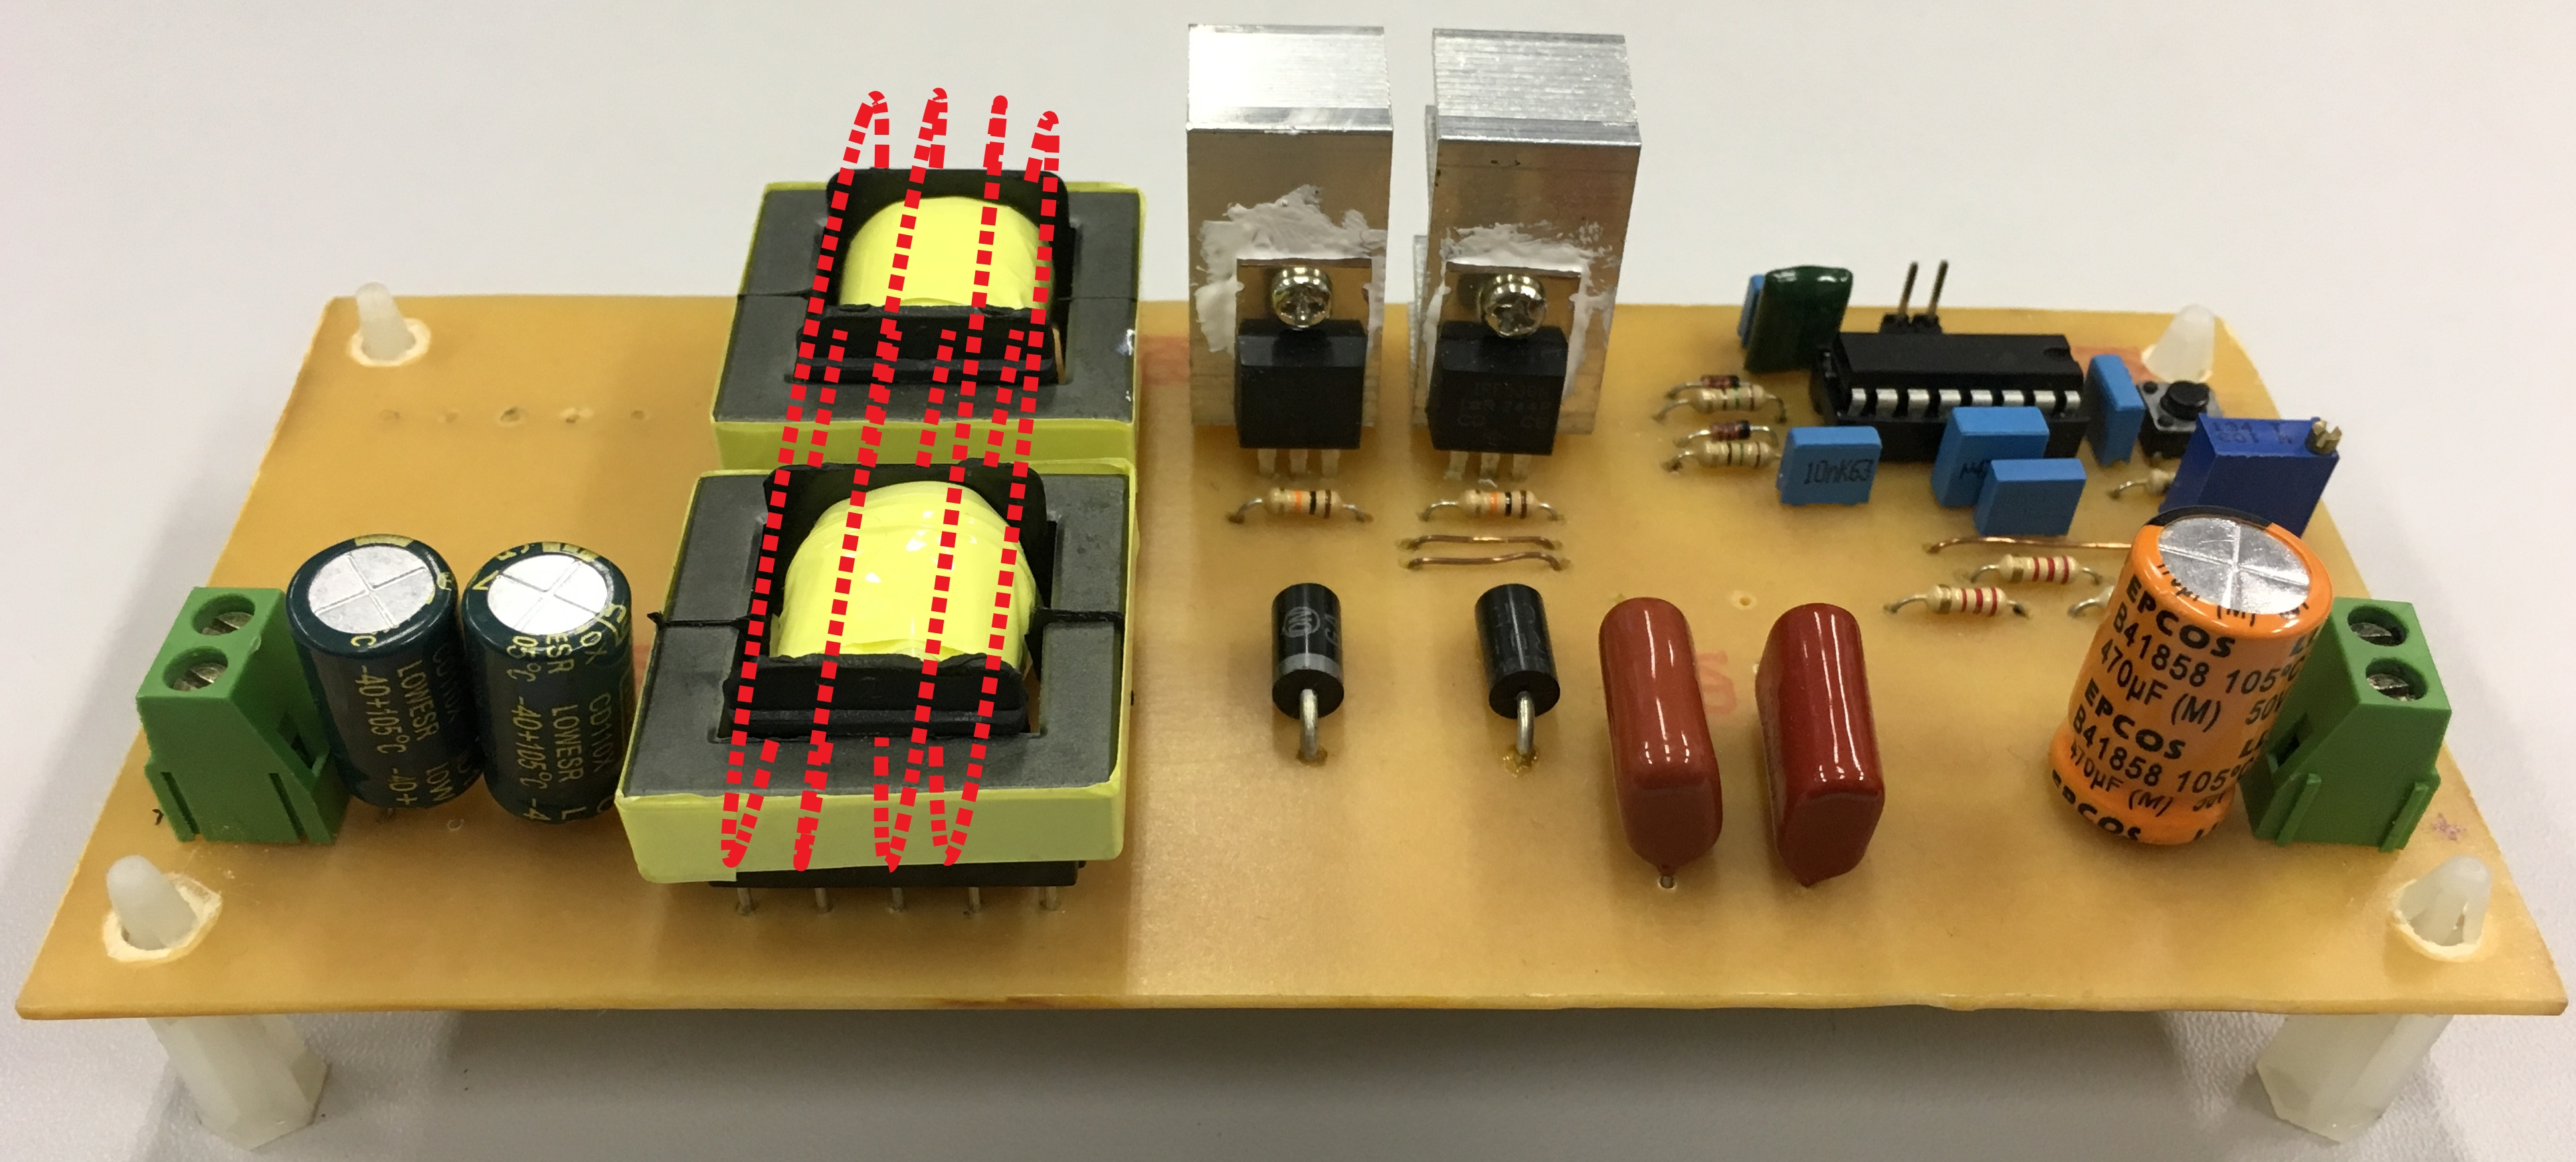
\includegraphics[scale=.1]{pdf/fotos/placa_vista_lateral_fluxo.jpg}
        \label{fig:foto_cbi_2}
     	\indentedfont[14cm]{Elaboração própria (2021)}
    \end{figure}
    
    Dessa forma, a mudança de posição de um dos indutores, como na \autoref{fig:foto_cbi_3}, proporciona uma mudança na direção do fluxo magnético disperso no ar, gerando um menor acoplamento entre ambos. 
    %um dos indutores presentes foi rotacionado, como mostra a \autoref{fig:foto_cbi_3}, buscando um menor acoplamento entre ambos. 
    
    \begin{figure}[H]
    	\centering
    	\caption{Representação da placa com um indutor rotacionado indutores no circuito inicial}
    	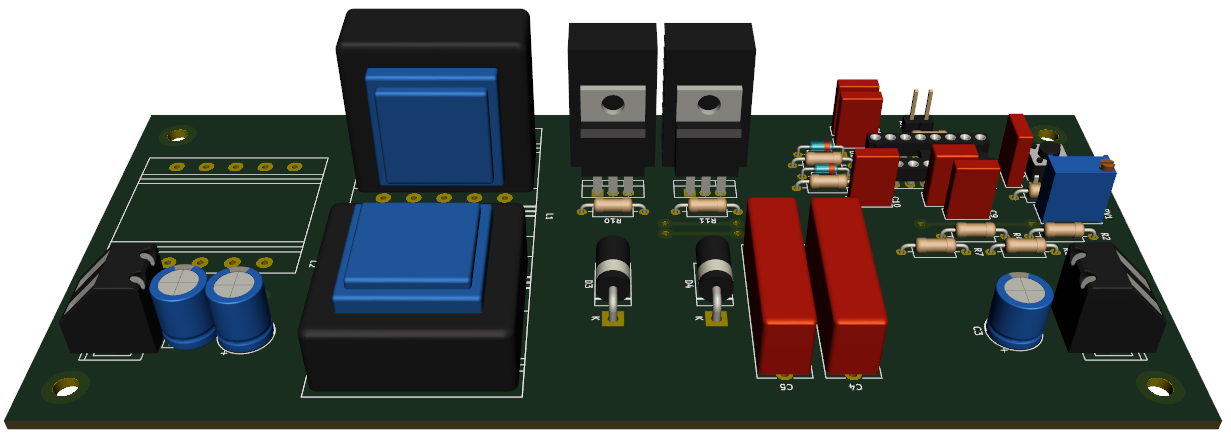
\includegraphics[scale=.3]{pdf/fotos/tecnica_indutor.png}
        \label{fig:foto_cbi_3}
     	\indentedfont[14cm]{Elaboração própria (2021)}
    \end{figure}
    
    O  comparativo da emissão conduzida entre os resultados obtidos para o circuito inicial e após o reposicionamento do indutor, pode ser observado na \autoref{fig:med_cond_indutor}.
    
    \begin{figure}[H]
    	\centering
    	\caption{Comparação dos resultados do ensaio de emissão conduzida para o circuito inicial e com um dos indutores rotacionado}
    	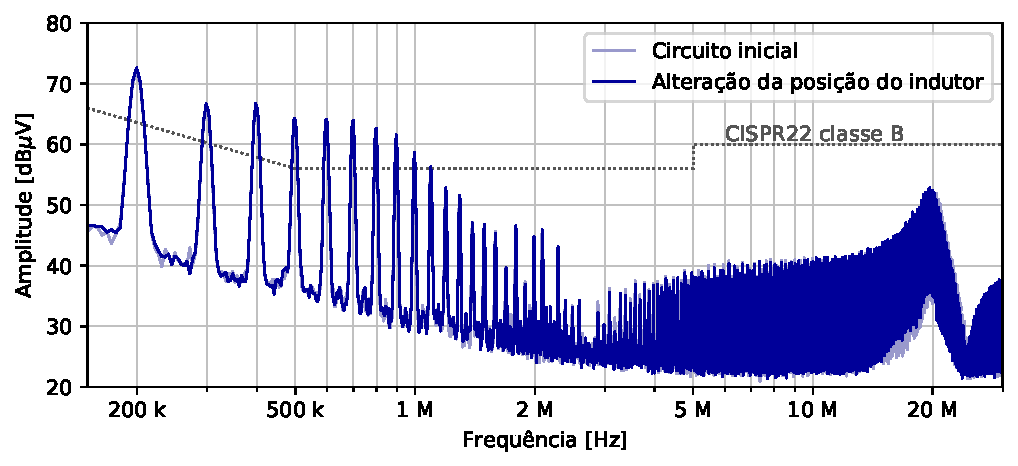
\includegraphics[scale=.9]{pdf/cond/Alteração da posição do indutor.pdf}
    	\label{fig:med_cond_indutor}
     	\indentedfont[15.5cm]{Elaboração própria (2021)}
    \end{figure}
    
    Observa-se que para a emissão conduzida não houve mudanças nos resultados. Na \autoref{fig:med_rad_indutor}, tem-se os resultados obtidos para a mesma técnica para a emissão irradiada. 
    
    \begin{figure}[H]
    	\centering
    	\caption{Comparação dos resultados do ensaio de emissão irradiada para o circuito inicial e com um dos indutores rotacionado}
    	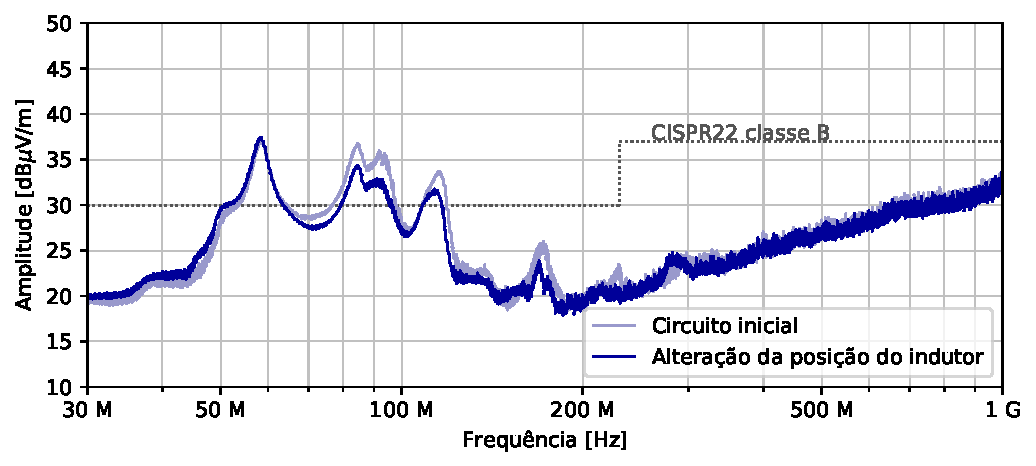
\includegraphics[scale=.9]{pdf/rad/Alteração da posição do indutor.pdf}
    	\label{fig:med_rad_indutor}
     	\indentedfont[15.5cm]{Elaboração própria (2021)}
    \end{figure}
    
    Nota-se uma pequena redução no entorno das frequências de \SI{85}{\mega\hertz}, \SI{93}{\mega\hertz}, \SI{115}{\mega\hertz}, \SI{170}{\mega\hertz} e \SI{230}{\mega\hertz}, que apesar de miníma, ainda torna-se relevante. 
    
    %%%%%%%%%%%%%%%%%%%%%%%%%%%%%%%%%%%%%%%%%%%%%%%%%%%%%%%%%%%%%%%%%%%
    \subsection{Técnica relacionada ao conversor 3SSC} \label{cap:result_tecnicas_3ssc}
    %%%%%%%%%%%%%%%%%%%%%%%%%%%%%%%%%%%%%%%%%%%%%%%%%%%%%%%%%%%%%%%%%%%
    
    A última técnica estudada neste trabalho foi a alteração da estrutura de um conversor Buck \interleaved para um conversor com célula de comutação de três estados. Nessa técnica o objetivo é utilizar a estrutura para reduzir a frequência de chaveamento, mantendo a dimensão dos elementos de filtro. 
    
    Nesse teste, optou-se pelo uso da frequência de chaveamento de \SI{20}{\kilo\hertz}, para que a frequência do harmônico fundamental do chaveamento esteja longe da faixa medida pelo teste de emissão conduzida. Para tal, alguns componentes presentes na PCB do circuito inicial precisam ser alterados, sendo eles: o indutor L3 deve ser adicionado, os indutores L1 e L2 devem ser substituídos por um autotransformador, os capacitores de saída (C6 e C7) devem ser calculados para a nova estrutura. A \autoref{fig:esquematico_cbi_5} apresenta, sem o circuito de acionamento, o circuito do conversor 3SSC utilizado. 
    
    \begin{figure}[H]
    	\centering
    	\caption{Esquemático simplificado utilizado do conversor 3SSC}
    	\includegraphics[scale=1.5]{pdf/layout/Esquematico_3ssc.pdf}
        \label{fig:esquematico_cbi_5}
     	\indentedfont[13.5cm]{Elaboração própria (2021)}
    \end{figure}
    
    Utilizando a \autoref{eq:3ssc_indutor} e a \autoref{eq:3ssc_capacitor}, calculou-se os novos valores de indutância e capacitância para a nova estrutura (para uma frequência de \SI{20}{\kilo\hertz}), obtendo os valores de \SI{36}{\micro\henry} e \SI{198}{\micro\farad}, respectivamente. Porém, devido a disponibilidade de capacitores de baixo valore de ESR, manteve-se os valores de capacitância já utilizados (dois capacitores eletrolíticos de \SI{470}{\micro\farad}). 
    
    Para minimizar os impactos gerados pela alteração do circuito, o indutor e o autotransformador projetados utilizaram o mesmo tipo de núcleo dos indutores do projeto inicial. Em todos os testes realizados com essa estrutura, os requisitos elétricos foram validados. 
    
    O modelo 3D da placa após as alterações no circuito, pode ser observado na \autoref{fig:3d_tecnica_3ssc}.
    
    \begin{figure}[H]
    	\centering
    	\caption{Modelo 3D do conversor desenvolvido convertido em conversor 3SSC}
    	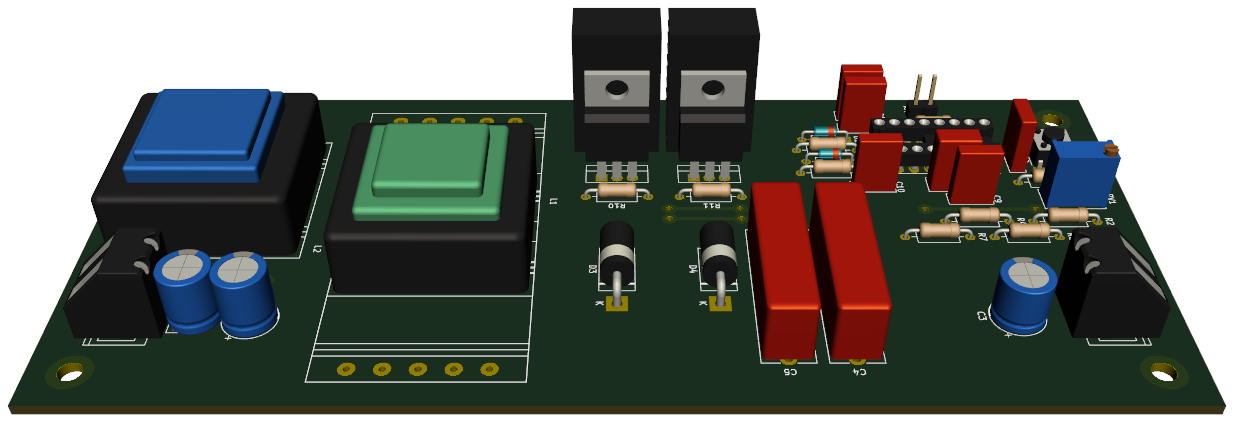
\includegraphics[scale=.35]{pdf/fotos/tecnica_3ssc.png}
        \label{fig:3d_tecnica_3ssc}
     	\indentedfont[15.5cm]{Elaboração própria (2021)}
    \end{figure}
    
    Assim, a \autoref{fig:med_cond_3ssc20k_EG} apresenta a comparação dos resultados obtidos da emissão conduzida para o circuito inicial (CBI) e para a nova estrutura (conversor 3SSC) em uma frequência de \SI{20}{\kilo\hertz}.
    
    %Com o objetivo de verificar seus impactos, a nova estrutura foi testada inicialmente em uma frequência de \SI{50}{\kilo\hertz}. A \autoref{fig:med_cond_3ssc50k} traz a comparação dos resultados obtidos da emissão conduzida para o circuito inicial (CBI) e para a nova estrutura (conversor 3SSC) em uma frequência de \SI{50}{\kilo\hertz}.
    
    %\begin{figure}[H]
    %	\centering
    %	\caption{Comparação dos resultados do ensaio de emissão conduzida para um CBI e um conversor 3SSC com uma frequência de chaveamento de \SI{50}{\kilo\hertz}}
    %	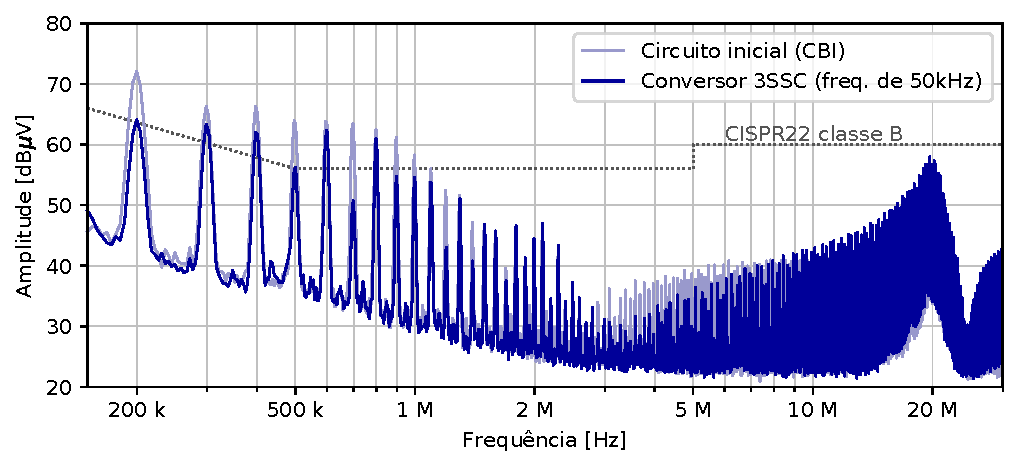
\includegraphics[scale=.9]{pdf/cond/Conversor 3SSC (freq. de 50kHz).pdf}
    %	\label{fig:med_cond_3ssc50k}
    % 	\indentedfont[15.5cm]{Elaboração própria (2021)}
    %\end{figure}
    
    %Percebe-se na figura que houve algumas alterações nos valores em alguns pontos medidos, porém os harmônicos de maior relevância se mantiveram os mesmos. O comparativo dos resultados da emissão irradiada para o mesmo teste pode ser observado na \autoref{fig:med_rad_3ssc50k}.
    
    %\begin{figure}[H]
    %	\centering
    %	\caption{Comparação dos resultados do ensaio de emissão irradiada para um CBI e um conversor 3SSC com uma frequência de chaveamento de \SI{50}{\kilo\hertz}}
    %	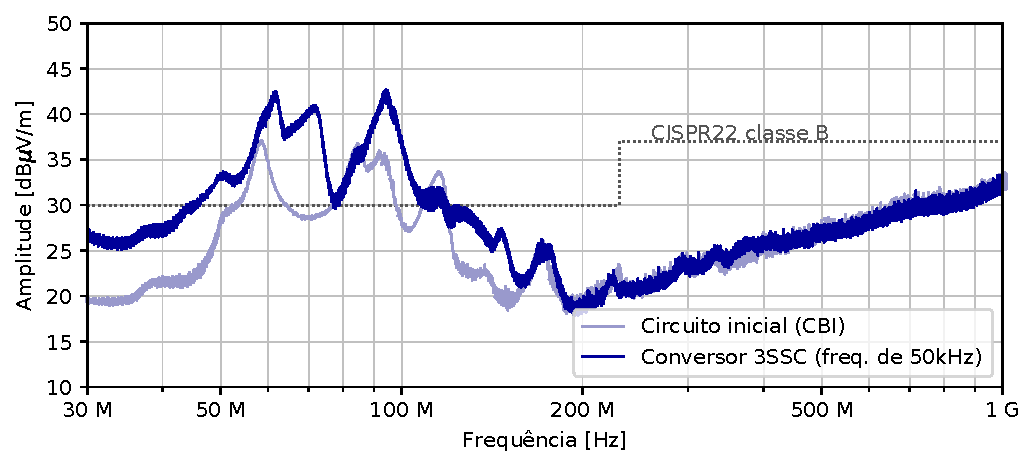
\includegraphics[scale=.9]{pdf/rad/Conversor 3SSC (freq. de 50kHz).pdf}
    %	\label{fig:med_rad_3ssc50k}
    % 	\indentedfont[15.5cm]{Elaboração própria (2021)}
    %\end{figure}
    
    %Como observado, apesar da redução dos valores na emissão conduzida, essa estrutura proporcionou um grande aumento nos valores obtidos na emissão irradiada. Percebe-se um aumento significativo nas frequências abaixo de \SI{170}{\mega\hertz}, com um novo pico no entorno de \SI{72}{\mega\hertz}.
    
    %Verificada as características da nova estrutura para a frequência de operação de \SI{50}{\kilo\hertz}, pode-se iniciar os testes para a frequência de projeto da nova estrutura, \SI{20}{\kilo\hertz}. Em todos os testes realizados com essa estrutura, os requisitos elétricos foram validados. Assim, a \autoref{fig:med_cond_3ssc20k_EG} apresenta a comparação dos resultados obtidos da emissão conduzida para o circuito inicial (CBI) e para a nova estrutura (conversor 3SSC) em uma frequência de \SI{20}{\kilo\hertz}.
    
    \begin{figure}[H]
    	\centering
    	\caption{Comparação dos resultados do ensaio de emissão conduzida para um CBI e um conversor 3SSC com uma frequência de chaveamento de \SI{20}{\kilo\hertz}}
    	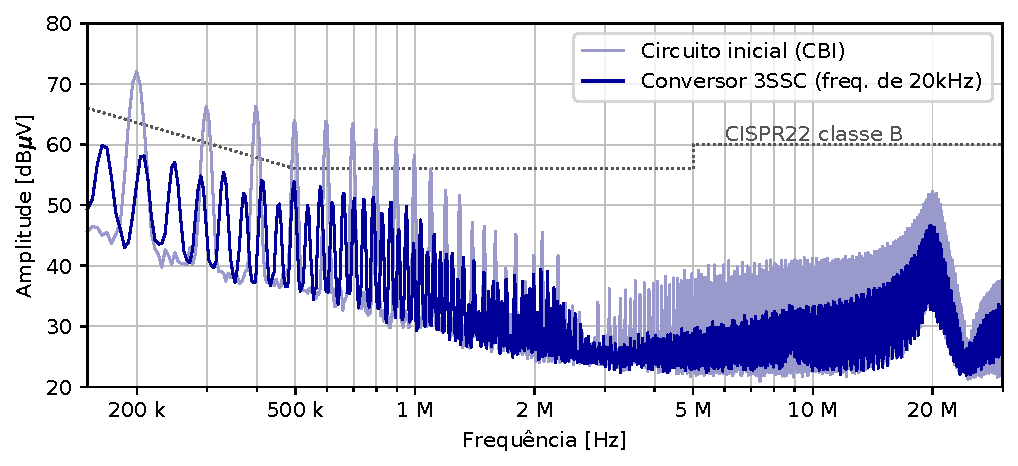
\includegraphics[scale=.9]{pdf/cond/Conversor 3SSC (freq. de 20kHz).pdf}
    	\label{fig:med_cond_3ssc20k_EG}
     	\indentedfont[15.5cm]{Elaboração própria (2021)}
    \end{figure}
    
    Nota-se nesse teste que, diferente das técnicas anteriores, foi possível reduzir consideravelmente os níveis de emissão conduzida em toda a faixa avaliada. 
    
    Na \autoref{fig:med_rad_3ssc20k_EG}, tem-se o comparativo dos resultados da emissão irradiada para o circuito inicial (CBI) e para a nova estrutura (conversor 3SSC) em uma frequência de \SI{20}{\kilo\hertz}.
    
    \begin{figure}[H]
    	\centering
    	\caption{Comparação dos resultados do ensaio de emissão irradiada para um CBI e um conversor 3SSC com uma frequência de chaveamento de \SI{20}{\kilo\hertz}}
    	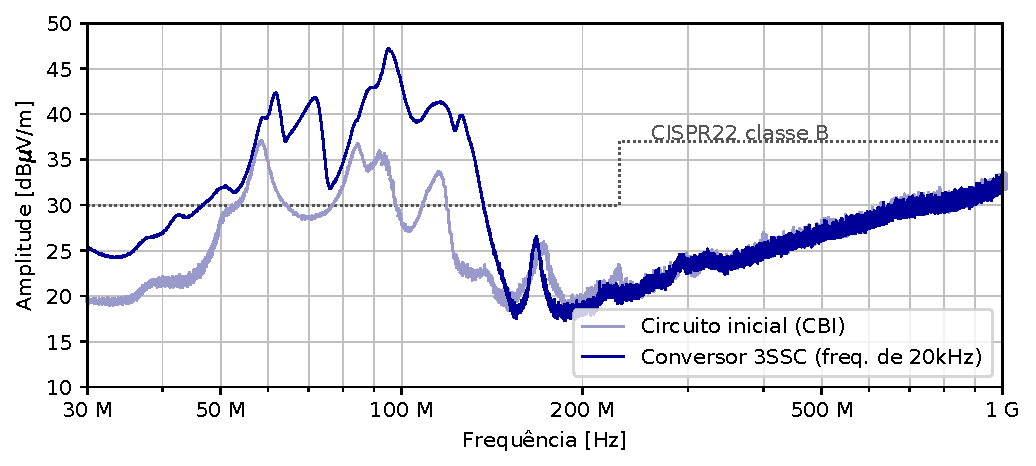
\includegraphics[scale=.9]{pdf/rad/Conversor 3SSC (freq. de 20kHz).pdf}
    	\label{fig:med_rad_3ssc20k_EG}
     	\indentedfont[15.5cm]{Elaboração própria (2021)}
    \end{figure}
    
    Diferente do teste de emissão conduzida, na emissão irradiada, houve um acréscimo nos níveis emitidos, para frequências inferiores \SI{170}{\mega\hertz}. 
    
    Durante os testes, percebeu-se que uma possível causa do aumento nos níveis de irradiação poderia ser o tamanho do entreferro escolhido para o indutor L3. Dessa forma, o indutor foi reprojetado, utilizando um entreferro menor, mantendo o seu valor de indutância. A \autoref{fig:med_cond_3ssc20k} apresenta a comparação dos resultados obtidos da emissão conduzida para o circuito inicial (CBI) e para a nova estrutura (conversor 3SSC) em uma frequência de \SI{20}{\kilo\hertz} para um entreferro reduzido.
    
    \begin{figure}[H]
    	\centering
    	\caption{Comparação dos resultados do ensaio de emissão conduzida para um CBI e um conversor 3SSC com uma frequência de chaveamento de \SI{20}{\kilo\hertz} para um entreferro reduzido}
    	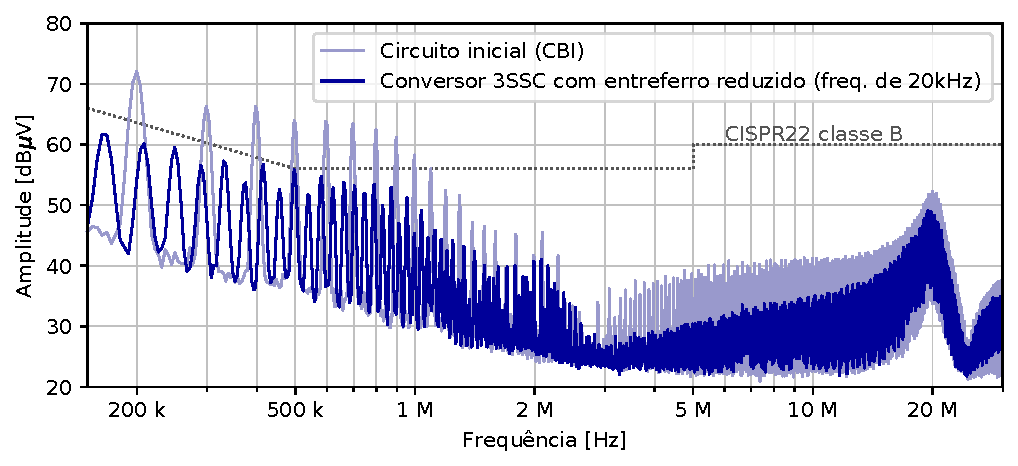
\includegraphics[scale=.9]{pdf/cond/Conversor 3SSC com entreferro reduzido (freq. de 20kHz).pdf}
    	\label{fig:med_cond_3ssc20k}
     	\indentedfont[15.5cm]{Elaboração própria (2021)}
    \end{figure}
    
    Na emissão conduzida não houve grandes mudanças nos resultados entre o entreferro grande e reduzido, como apresentado na \autoref{fig:med_cond_3ssc_comp}, ficando seus valores de pico muito próximos.
    
    \begin{figure}[H]
    	\centering
    	\caption{Comparação dos resultados do ensaio de emissão conduzida entre um conversor 3SSC com uma frequência de chaveamento de \SI{20}{\kilo\hertz} para um entreferro grande e um entreferro reduzido}
    	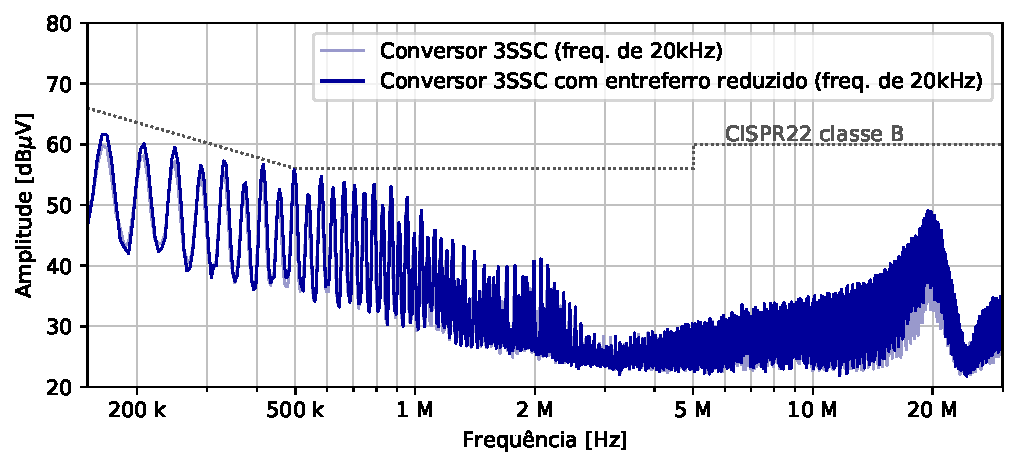
\includegraphics[scale=.9]{pdf/cond/cond-Conversor 3SSC (freq. de 20kHz)-Conversor 3SSC com entreferro reduzido (freq. de 20kHz).pdf}
    	\label{fig:med_cond_3ssc_comp}
     	\indentedfont[15.5cm]{Elaboração própria (2021)}
    \end{figure}
    
    Porém, para a emissão irradiada nos resultados entre o entreferro grande e reduzido, \autoref{fig:med_rad_3ssc20k}, houveram mudanças maiores. 
    
    \begin{figure}[H]
    	\centering
    	\caption{Comparação dos resultados do ensaio de emissão irradiada para um CBI e um conversor 3SSC com uma frequência de chaveamento de \SI{20}{\kilo\hertz} para um entreferro reduzido}
    	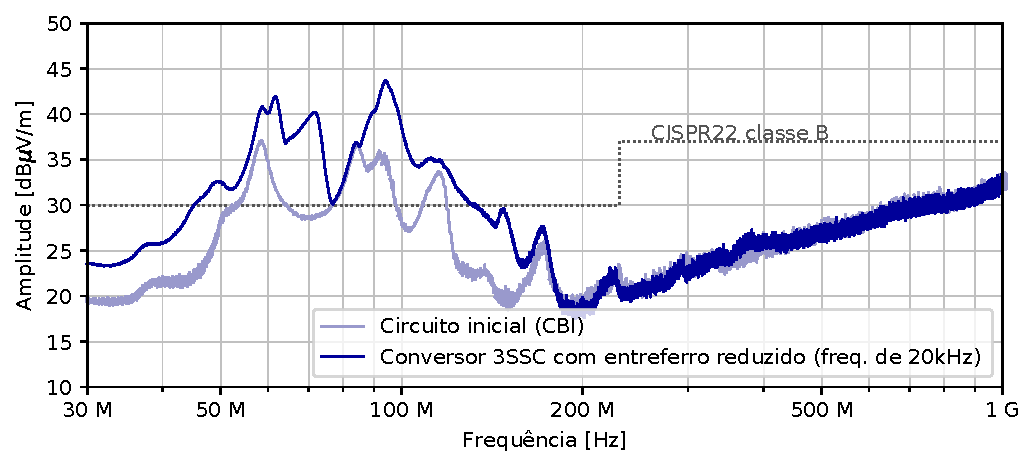
\includegraphics[scale=.9]{pdf/rad/Conversor 3SSC com entreferro reduzido (freq. de 20kHz).pdf}
    	\label{fig:med_rad_3ssc20k}
     	\indentedfont[15.5cm]{Elaboração própria (2021)}
    \end{figure}
    
    Pela figura, percebe-se que, apesar dos maiores picos, se comparado ao CBI inicial, há uma menor emissão irradiada se comparado ao conversor 3SSC com o entreferro grande. Essa diferença entre a emissão irradiada do conversor 3SSC com o indutor com entreferro grande e com o entreferro reduzido pode ser observado na \autoref{fig:med_rad_3ssc_comp}. 
    
    \begin{figure}[H]
    	\centering
    	\caption{Comparação dos resultados do ensaio de emissão irradiada entre um conversor 3SSC com uma frequência de chaveamento de \SI{20}{\kilo\hertz} para um entreferro grande e um entreferro reduzido}
    	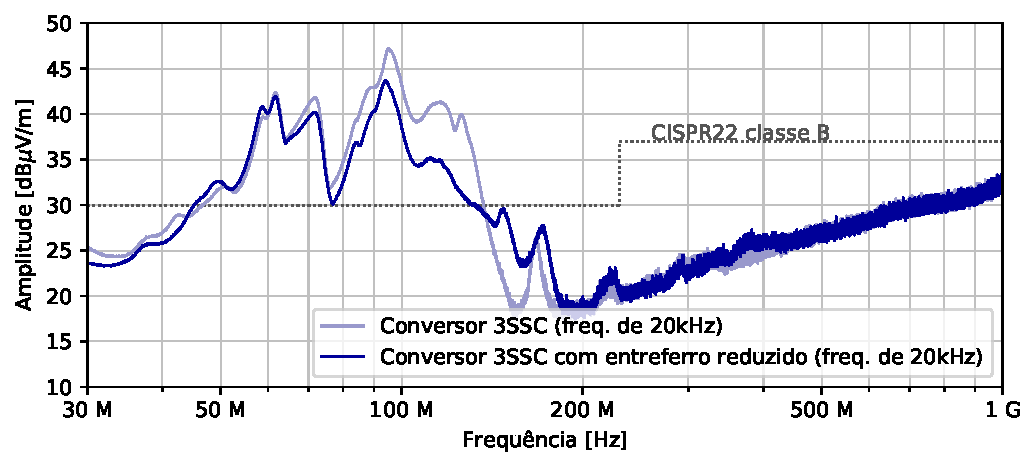
\includegraphics[scale=.9]{pdf/rad/rad-Conversor 3SSC (freq. de 20kHz)-Conversor 3SSC com entreferro reduzido (freq. de 20kHz).pdf}
    	\label{fig:med_rad_3ssc_comp}
     	\indentedfont[15.5cm]{Elaboração própria (2021)}
    \end{figure}
    
    Na figura, nota-se uma redução nos níveis emitidos entre as frequências de \SI{80}{\mega\hertz} e \SI{200}{\mega\hertz} devido a mudança no entreferro do indutor. Assim, apesar da redução nos níveis de emissão conduzida para essa estrutura, há um aumento na emissão irradiada. Ainda, percebe-se a necessidade de um grande cuidado ao projetar os indutores, uma vez que seu entreferro é um dos grandes responsáveis pela emissão irradiada. 
    
    % DIc = 2.0377 -> L = 35,78uH
    % 29,17uH
    % 198uF
    
    %%%%%%%%%%%%%%%%%%%%%%%%%%%%%%%%%%%%%%%%%%%%%%%%%%%%%%%%%%%%%%%%%%%
    \subsection{Uso combinado das técnicas com melhores resultados} \label{cap:result_tecnicas_total}
    %%%%%%%%%%%%%%%%%%%%%%%%%%%%%%%%%%%%%%%%%%%%%%%%%%%%%%%%%%%%%%%%%%%
    
    O uso do conversor 3SSC, apesar de apresentar maiores níveis de emissão irradiada, consiste em uma boa alternativa para a redução da emissão conduzida, podendo até substituir o uso de filtros como técnica. Aliado ao conversor 3SSC, algumas técnicas e soluções de mitigação de emissão irradiada podem ser aplicadas, buscando um equilíbrio entre as emissões. 
    
    Assim, buscando demonstrar a viabilidade das técnicas estudadas, aplicou-se uma combinação das técnicas com melhor resultado junto ao conversor 3SSC. Dessa forma, foi utilizado a técnica de uso de um núcleo de ferrite nos terminais de dreno dos transistores e a conexão dos dissipadores á referência do circuito com um capacitor de \SI{100}{\nano\farad}. A \autoref{fig:med_cond_todas_tec} apresenta o comparativo entre os resultados do ensaio de emissão conduzida do circuito inicial (CBI) e o uso das técnicas com melhores resultados (uso de um núcleo de ferrite no terminal de dreno + conexão dos dissipadores à referência + conversor 3SSC com frequência de operação de \SI{20}{\kilo\hertz}).
    
    \begin{figure}[H]
    	\centering
    	\caption{Comparação entre os resultados do ensaio de emissão conduzida do circuito inicial e o uso das técnicas com melhores resultados}
    	\includegraphics[scale=.9]{pdf/cond/Uso das melhores técnicas.pdf}
    	\label{fig:med_cond_todas_tec}
     	\indentedfont[15.5cm]{Elaboração própria (2021)}
    \end{figure}
    
    Percebe-se pela figura, que apesar de não ser o objetivo desse estudo, o uso das técnicas combinadas foram capazes de colocar o conversor proposto abaixo dos níveis estabelecidos pela norma CISPR22 classe B de emissão conduzida. A \autoref{fig:med_rad_todas_tec} apresenta o comparativo da emissão irradiada para o mesmo teste. 
    
    \begin{figure}[H]
    	\centering
    	\caption{Comparação entre os resultados do ensaio de emissão irradiada do circuito inicial e o uso das técnicas com melhores resultados}
    	\includegraphics[scale=.9]{pdf/rad/Uso das melhores técnicas.pdf}s
    	\label{fig:med_rad_todas_tec}
     	\indentedfont[15.5cm]{Elaboração própria (2021)}
    \end{figure}
    
    Um resultado semelhante a emissão conduzida pode ser observado nessa figura, que apesar do aumento na emissão irradiada provocada pelo conversor 3SSC, as demais técnicas utilizadas foram capazes de contrabalancear essa emissão. Percebe-se que há uma grande redução nos níveis medidos em toda a faixa avaliada na norma, com apenas alguns poucos pontos acima dos limites estabelecidos por ela. 
    
    % TABELA RESUMO DE QUAIS FREQUÊNCIAS REDUZIRAM E AUMENTARAM COM QUAIS TÉCNICAS
    
\chapter{Considerações Finais}
    No desenvolvimento de um conversor estático para fins comerciais, alguns cuidados do ponto de vista de EMC devem ser tomados pelo projetista, uma vez que o seu produto deve passar por algumas normas para que tenha permissão para comercialização. 
    
    Há diversas técnicas para soluções de problemas de EMC disponíveis para os diversos tipos de aplicações, tanto para a emissão conduzida quanto para a emissão irradiada. Dentre elas, algumas foram avaliadas neste trabalho, de forma isolada, em um conversor estático CC-CC do tipo Buck \interleaved. Os resultados obtidos mostraram-se interessantes, com nenhuma das técnicas mostrando-se uma solução perfeita para os problemas presentes, solucionando em determinadas faixas de frequências e sendo irrelevantes ou menos eficazes em outras. Porém, ao utilizar uma combinação das mesmas, resultados ainda mais interessantes podem ser obtidos, com melhoras tanto da emissão conduzida quanto da emissão irradiada. 
    
    Dentre as técnicas propostas, destacaram-se pela redução do ruído irradiado o uso de capacitores para a conexão dos dissipadores a referência do circuito e o uso de um núcleo de ferrite nos terminais de dreno dos transistores. Já no ensaio de emissão conduzida, a redução da frequência de chaveamento através do conversor 3SSC foi de grande destaque. Durante todos os testes, realizou-se medidas elétricas no circuito, avaliando o impacto das técnicas no seu funcionamento. Nesses testes verificou-se que não houve alterações no funcionamento, mantendo o conversor dentro dos requisitos estabelecidos.
    
    Durante o trabalho, o uso da padronização da posição dos cabos e da placa foi de grande valia, uma vez que a sua variação durante a medição de emissão irradiada ocasionava em uma grande mudança nos valores medidos. Para o projeto dos indutores, a variação do tamanho do entreferro foi de grande influência na emissão irradiada, e é um fator que muitas vezes não recebe a devida atenção pelos projetistas. 
    
    Apesar das diversas técnicas de EMC apresentadas nesse projeto, muitas outras ainda podem ser estudadas no conversor proposto ou variações das mesmas. Uma delas é a conexão dos dissipadores a referência sem o uso de um capacitor, desde que seja feito o seu isolamento, e o uso de capacitores de diferentes valores de capacitância. Dessa forma, pode-se avaliar melhor o impacto da capacitância escolhida na redução das emissões. 
    
    Também, mostra-se relevante para estudos futuros um melhor estudo do impacto do entreferro dos indutores na emissão irradiada, podendo ser estudado tanto a variação do entreferro quanto a mudança dos tipos de núcleo. Ainda, sugere-se um maior estudo do conversor 3SSC, com uma análise em diferentes frequências, tanto do ponto de vista da compatibilidade eletromagnética quanto do ponto de vista de potência.
    
    Assim, com todos os objetivos propostos alcançados, este trabalho buscou agregar conhecimento para os próximos trabalhos na área, tanto para os estudos de conversores Buck \interleaved e conversores com 3SSC quanto no estudo da EMI.
    
    

% ----------------------------------------------------------
% ELEMENTOS PÓS-TEXTUAIS
% ----------------------------------------------------------
\postextual
% ----------------------------------------------------------

% ----------------------------------------------------------
% Referências bibliográficas
% ----------------------------------------------------------
\bibliography{referencias}

% ----------------------------------------------------------
% Apêndices
% ----------------------------------------------------------
\begin{apendicesenv}
    \partapendices
    \chapter{Componentes usados no Buck \interleaved}
%\addcontentsline{toc}{part}{Introdução}

    \begin{table}[htbp]
        \centering
        %\caption{Especificações de projeto do conversor Buck \Interleaved de dois ramos}
        %\label{tab:componentes}
        \begin{tabular}{@{}|m{0.08\textwidth}|m{0.30\textwidth}|m{0.50\textwidth}|@{}}
            \hline
            ID & Componente & Valor \\
            \hline
            R1  &   Resistor PTH                &   \qty{10}{\kilo$\Omega$} $\pm$ \qty{5}{\percent}\\ %\hline
            R2	&	Resistor PTH	            &	\qty{10}{\kilo$\Omega$} $\pm$ \qty{5}{\percent}\\
            R3	&	Resistor PTH	            &	\qty{1.2}{\kilo$\Omega$} $\pm$ \qty{5}{\percent}\\
            R4	&	Resistor PTH	            &	\qty{2}{\kilo$\Omega$} $\pm$ \qty{5}{\percent}\\
            R6	&	Resistor PTH	            &	\qty{820}{$\Omega$} $\pm$ \qty{5}{\percent}\\
            R7	&	Resistor PTH	            &	\qty{2}{\kilo$\Omega$} $\pm$ \qty{5}{\percent}\\
            R8	&	Resistor PTH	            &	\qty{22}{$\Omega$} $\pm$ \qty{5}{\percent}\\
            R9	&	Resistor PTH	            &	\qty{22}{$\Omega$} $\pm$ \qty{5}{\percent}\\
            R10	&	Resistor PTH	            &	\qty{10}{\kilo$\Omega$} $\pm$ \qty{5}{\percent}\\
            R11	&	Resistor PTH	            &	\qty{10}{\kilo$\Omega$} $\pm$ \qty{5}{\percent}\\
            RV1	&	Potenciômetro multivoltas	&	\qty{10}{\kilo$\Omega$} \\
            C1	&	Capacitor de poliéster	    &	\qty{10}{\nano\farad} $\pm$ \qty{20}{\percent}\\
            C2	&	Capacitor de poliéster	    &	\qty{470}{\nano\farad} $\pm$ \qty{20}{\percent}\\
            C3	&	Capacitor de eletrolítico	&	\qty{100}{\micro\farad} $\pm$ \qty{20}{\percent}\\
            C4	&	Capacitor de poliéster	    &	\qty{470}{\micro\farad} $\pm$ \qty{20}{\percent}\\
            C5	&	Capacitor de poliéster	    &	\qty{470}{\micro\farad} $\pm$ \qty{20}{\percent}\\
            C6	&	Capacitor de eletrolítico	&	\qty{470}{\micro\farad} $\pm$ \qty{20}{\percent}\\
            C7	&	Capacitor de eletrolítico	&	\qty{470}{\micro\farad} $\pm$ \qty{20}{\percent}\\
            C8	&	Capacitor de poliéster	    &	\qty{10}{\nano\farad} $\pm$ \qty{20}{\percent}\\
            C9	&	Capacitor de poliéster	    &	\qty{100}{\nano\farad} $\pm$ \qty{20}{\percent}\\
            C10	&	Capacitor de poliéster	    &	\qty{10}{\nano\farad} $\pm$ \qty{20}{\percent}\\
            C11	&	Capacitor de poliéster	    &	\qty{1}{\micro\farad} $\pm$ \qty{20}{\percent}\\
            D1	&	Diodo rápido                &	1N4148\\
            D2	&	Diodo rápido                &	1N4148\\
            D3	&	Diodo ultra-fast            &	MUR460\\
            D4	&	Diodo ultra-fast            &	MUR460\\
            Q1	&	MOSFET de potência          &	IRF540N\\
            Q2	&	MOSFET de potência          &	IRF540N\\
            U1	&	Circuito de controle PWM    &	SG3525\\
            L1	&	Indutor             	    &	\qty{31}{\micro\henry} - 16 Espiras com 2 fios p. AWG22  \\
            L2	&	Indutor             	    &	\qty{31}{\micro\henry} - 16 Espiras com 2 fios p. AWG22  \\
            N   &	Núcleo de L1 e L2           &	Núcleo Magmattec de ferrite 140 do tipo Mn-Zn EE-30/7 \\
            \hline
        \end{tabular}
        \indentedfont[0.96\textwidth]{Elaboração própria (2021)}
    \end{table}

\chapter{Componentes usados durante as técnicas}

    \begin{table}[htbp]
        \centering
        %\caption{Especificações de projeto do conversor Buck \Interleaved de dois ramos}
        %\label{tab:componentes_tec}
        \begin{tabular}{@{}|m{0.08\textwidth}|m{0.30\textwidth}|m{0.50\textwidth}|@{}}
            \hline
            ID & Componente & Valor \\
            \hline
            R8	&	Resistor PTH	            &	\qty{68}{$\Omega$} $\pm$ \qty{5}{\percent}\\
            R9	&	Resistor PTH	            &	\qty{68}{$\Omega$} $\pm$ \qty{5}{\percent}\\
            $C_D$	&	Capacitor cerâmico	    &	\qty{1}{\nano\farad} $\pm$ \qty{20}{\percent}\\
            $C_D$	&	Capacitor cerâmico	    &	\qty{100}{\nano\farad} $\pm$ \qty{20}{\percent}\\
            L   &   Núcleo de Ferrite (Bead)    &   Ferrite Bead com material IP6\\
            L3	&	Indutor do conv. 3SSC       &	\qty{36}{\micro\henry} - 17 Espiras com 4 fios p. AWG22 \\
            T	&	Autotransformador           &	7 Espiras com 2 fios AWG22 em paralelo \\
            N   &	Núcleo L3 e T   	        &	Núcleo Magmattec de ferrite 140 do tipo Mn-Zn EE-30/7 \\
            \hline
        \end{tabular}
        \indentedfont[0.96\textwidth]{Elaboração própria (2021)}
    \end{table}
\end{apendicesenv}

% ----------------------------------------------------------
% Anexos
% ----------------------------------------------------------
%\begin{anexosenv}
%    \partanexos
%    \chapter{Meu primeiro assunto de anexo}


\chapter{Segundo assunto que pesquisei}

%\end{anexosenv}

%---------------------------------------------------------------------
% INDICE REMISSIVO
%---------------------------------------------------------------------
%\phantompart
%\printindex
%---------------------------------------------------------------------

\end{document}
